\documentclass[journal]{IEEEtran}






% *** GRAPHICS RELATED PACKAGES ***
%
\ifCLASSINFOpdf
  % \usepackage[pdftex]{graphicx}
  % declare the path(s) where your graphic files are
  % \graphicspath{{../pdf/}{../jpeg/}}
  % and their extensions so you won't have to specify these with
  % every instance of \includegraphics
  % \DeclareGraphicsExtensions{.pdf,.jpeg,.png}
\else
  % or other class option (dvipsone, dvipdf, if not using dvips). graphicx
  % will default to the driver specified in the system graphics.cfg if no
  % driver is specified.
  % \usepackage[dvips]{graphicx}
  % declare the path(s) where your graphic files are
  % \graphicspath{{../eps/}}
  % and their extensions so you won't have to specify these with
  % every instance of \includegraphics
  % \DeclareGraphicsExtensions{.eps}
\fi



\usepackage{setspace}
\usepackage{epsfig}  % for figures
\usepackage{epstopdf}
\usepackage{hyperref}

\usepackage{amssymb,amsmath,amsthm, mathtools}
\usepackage{mathrsfs} 

\let\labelindent\relax
\usepackage{enumitem}
\usepackage{subfiles}

\usepackage{caption}
\usepackage{subcaption}
\captionsetup{font=footnotesize}



\makeatletter
\newcommand{\removelatexerror}{\let\@latex@error\@gobble}
\makeatother
\usepackage{xcolor}
\usepackage[ruled, vlined]{algorithm2e}
\newcommand\mycommfont[1]{\footnotesize\em\textcolor{blue}{#1}}
\SetCommentSty{mycommfont}

\SetAlFnt{\small}

\usepackage{lipsum}
\usepackage{cite}
\usepackage{thmtools,thm-restate}
\usepackage{multicol}
\usepackage{bm}
%\theoremstyle{definition}
\newtheorem{definition}{Definition}[section]
\newtheorem{proposition}{Proposition}[section]
\newtheorem{lemma}{Lemma}[section]
\newtheorem{example}{Example}[section]
\newtheorem{theorem}{Theorem}[section]
\newtheorem{alg}{Algorithm}[section]
\newtheorem{corollary}{Corollary}[section]
%\theoremstyle{remark}
\newtheorem{remark}{Remark}[section]
\newtheorem{assumption}{Assumption}[section]
\newtheorem{conjecture}{Conjecture}[section]
\newtheorem{claim}{Claim}[section]
\newtheorem{property}{Property}[section]
\newtheorem{condition}{Condition}[section]
\newcommand{\vect}[1]{\boldsymbol{#1}}

\renewcommand\thetheorem{\arabic{section}.\arabic{theorem}}
\renewcommand\theproposition{\arabic{section}.\arabic{proposition}}
\renewcommand\thelemma{\arabic{section}.\arabic{lemma}}
\renewcommand\thecorollary{\arabic{section}.\arabic{corollary}}
\renewcommand\theconjecture{\arabic{section}.\arabic{conjecture}}
\renewcommand\thedefinition{\arabic{section}.\arabic{definition}}
\renewcommand\thecondition{\arabic{section}.\arabic{condition}}
\renewcommand\theassumption{\arabic{section}.\arabic{assumption}}
\renewcommand\thealg{\arabic{section}.\arabic{alg}}

\newcommand{\conv}{\textup{conv}}
\newcommand{\specificthanks}[1]{\@fnsymbol{#1}}% Inserts a specific \thanks symbol
\newcommand{\vertiii}[1]{{\left\vert\kern-0.25ex\left\vert\kern-0.25ex\left\vert #1 
    \right\vert\kern-0.25ex\right\vert\kern-0.25ex\right\vert}}

\DeclareMathOperator*{\argmin}{arg\,min}
\DeclareMathOperator*{\argmax}{arg\,max}


% SETH'S MATH
\providecommand{\sW}{\mathcal{W}}
\providecommand{\sF}{F}
\providecommand{\sP}{\mathcal{P}}
\providecommand{\sL}{\mathcal{L}}
\providecommand{\sN}{\widetilde{\mathcal{N}}}
\providecommand{\Tcs}{T^{\textup{cc}}}
\providecommand{\Tc}{\widetilde{T}^{\textup{cc}}}
\providecommand{\lyap}{\mathcal{L}}
\providecommand{\Tdl}{T^{\textup{dl}}}
\providecommand{\Tdlk}{T^{\textup{rd}}}
\newcommand{\diam}{\textup{diam}}
\newcommand{\M}{\bm{M}}
\newcommand{\A}{\bm{A}}
\newcommand{\HM}{\bm{H}}
\renewcommand{\thefootnote}{\arabic{footnote}}

%% NEW NOTATIONS!

\newcommand{\identity}{\bm{I}}
\newcommand{\barI}{\overline{I}}
%\newcommand{\barX}{\overline{x}}
\newcommand{\barX}{\overline{\bm{x}}}
\newcommand{\barG}{\overline{\mathcal{G}}}
\newcommand{\barV}{\overline{\mathcal{V}}}
\newcommand{\barE}{\overline{\mathcal{E}}}
\newcommand{\barN}{\overline{\mathcal{N}}_i}
\newcommand{\barn}{\overline{n}}
\newcommand{\nfmax}{\widetilde{n}_{f_i}}
\newcommand{\nfi}{{n}_{f_i}}
\newcommand{\gcup}{\widetilde{\mathcal{G}}}

% correct bad hyphenation here
\hyphenation{op-tical net-works semi-conduc-tor}


\begin{document}
	
	

%
% paper title
% Titles are generally capitalized except for words such as a, an, and, as,
% at, but, by, for, in, nor, of, on, or, the, to and up, which are usually
% not capitalized unless they are the first or last word of the title.
% Linebreaks \\ can be used within to get better formatting as desired.
% Do not put math or special symbols in the title.
\title{
	 Spatial Distribution Mapping by Mobile Sensor Networks: A Bayesian Method
}
%
%
% author names and IEEE memberships
% note positions of commas and nonbreaking spaces ( ~ ) LaTeX will not break
% a structure at a ~ so this keeps an author's name from being broken across
% two lines.
% use \thanks{} to gain access to the first footnote area
% a separate \thanks must be used for each paragraph as LaTeX2e's \thanks
% was not built to handle multiple paragraphs
%

\author{Hyongju~Park, Matthew~Johnson-Roberson and Ram~Vasudevan
        }% <-this % stops a space
%\thanks{Hyongju Park is with the Department
%		of Mechanical Science and Engineering, University of Illinois at Urbana-Champaign, Urbana,
%		IL, 61801 USA {\tt\small park334@illinois.edu}.}% <-this % stops a space
%\thanks{Seth A. Hutchinson is with the Department
%of Electrical and Computer Engineering, University of Illinois at Urbana-Champaign, Urbana,
%IL, 61801 USA {\tt\small seth@illinois.edu}.}% <-this % stops a space
%\thanks{Manuscript received August 19, 2015; revised September 17, 2015.}}

% note the % following the last \IEEEmembership and also \thanks - 
% these prevent an unwanted space from occurring between the last author name
% and the end of the author line. i.e., if you had this:
% 
% \author{....lastname \thanks{...} \thanks{...} }
%                     ^------------^------------^----Do not want these spaces!
%
% a space would be appended to the last name and could cause every name on that
% line to be shifted left slightly. This is one of those "LaTeX things". For
% instance, "\textbf{A} \textbf{B}" will typeset as "A B" not "AB". To get
% "AB" then you have to do: "\textbf{A}\textbf{B}"
% \thanks is no different in this regard, so shield the last } of each \thanks
% that ends a line with a % and do not let a space in before the next \thanks.
% Spaces after \IEEEmembership other than the last one are OK (and needed) as
% you are supposed to have spaces between the names. For what it is worth,
% this is a minor point as most people would not even notice if the said evil
% space somehow managed to creep in.



% The paper headers
%\markboth{Journal of \LaTeX\ Class Files,~Vol.~13, No.~9, September~2015}%
%{Shell \MakeLowercase{\textit{et al.}}: Bare Demo of IEEEtran.cls for Journals}
% The only time the second header will appear is for the odd numbered pages
% after the title page when using the twoside option.
% 
% *** Note that you probably will NOT want to include the author's ***
% *** name in the headers of peer review papers.                   ***
% You can use \ifCLASSOPTIONpeerreview for conditional compilation here if
% you desire.




% If you want to put a publisher's ID mark on the page you can do it like
% this:
%\IEEEpubid{0000--0000/00\$00.00~\copyright~2014 IEEE}
% Remember, if you use this you must call \IEEEpubidadjcol in the second
% column for its text to clear the IEEEpubid mark.



% use for special paper notices
%\IEEEspecialpapernotice{(Invited Paper)}




% make the title area
\maketitle

% As a general rule, do not put math, special symbols or citations
% in the abstract or keywords.
\begin{abstract}
The Fukushima Daiichi Nuclear Power Plant (NPP) incident resulted in a heavy radiation which has hampered recovery operations for years. Real-time mapping of the spatial distribution of radioactivity near and around reactors will assist safe and cost effective restoration and prevent further contamination, which aligns with the IAEA's continuous technical support on radiation monitoring. Such environmental mapping tasks can be done efficiently via dispatching a group of unmanned vehicles equipped with radiation sensors. This paper presents a Bayesian approach to estimating spatially distributed target maps by deploying a group of mobile robots, as motivated by the example.
The topological (locations) and spatial properties (e.g., radiation level, magnetic field strength, temperature levels, etc) which constitute the target state are unknown and are characterized by prior probability distribution over bounded domain.
This paper considers a continuous target domain, and robots that are equipped with noisy range sensors whose ability to detect the target varies probabilistically as a function of the distance between the robot and target.
We propose a deterministic motion model where robots move to maximize the observation likelihood based on the sensor measurements and prior beliefs on target state. In addition, we present a decentralized counterpart, suitable for short range sensors, where the workspace is partitioned into multiple disjoint regions, and each robot detects target only in its associated region.
Belief on target state is evolved by a variant of a classical Recursive Bayesian Filter. 
Computing the belief propagation is generally intractable for an arbitrary target distribution due 
to its non-modal characteristics. An approximation scheme are developed that exploits a standardized particle filtering method.
Both simulation results and real-world validation are presented to
demonstrate the effectiveness of the proposed methods.
\end{abstract}

% Note that keywords are not normally used for peerreview papers.
%\begin{IEEEkeywords}
%multi-robot system, fault-tolerant algorithm, order$-k$ Voronoi diagram, coverage control, deployment.
%\end{IEEEkeywords}
%




% For peer review papers, you can put extra information on the cover
% page as needed:
% \ifCLASSOPTIONpeerreview
% \begin{center} \bfseries EDICS Category: 3-BBND \end{center}
% \fi
%
% For peerreview papers, this IEEEtran command inserts a page break and
% creates the second title. It will be ignored for other modes.
\IEEEpeerreviewmaketitle


\section{Introduction}
\label{sec:sec1}
A large number of mobile robots equipped with ad-hoc communication and sensing devices, so called, Mobile Sensor Networks (MSNs) have a wide range of applications, including, exploration, surveillance, search and rescue missions, environmental
monitoring for pollution detection and estimation, target tracking, cooperative detection of hazardous materials in contaminated environments, forest fire monitoring, oceanographic modeling, etc \cite{dhillon2003sensor,howard2002mobile,cortes_coverage_2004,yu2005real}. In the past decade, estimating the unknown, spatially distributed target of interest (e.g., gas, odor, temperature, radiation, fume, etc) have received much attention from not only environmental scientists \cite{chuvieco1996mapping} but also from roboticists \cite{cortez2008smart,choi2010continuous,ristic2010information}. This finds numerous applications, including environmental monitoring, pollution detection, data collection tasks, etc.
MSNs have been shown to be ideal for such missions in that each sensors can move together and take measurements in-between or along their motions.
This paper aims to develop a class of sensing and motion model for MSNs to collectively obtain an accurate representation of an arbitrary spatial target map under the Bayesian framework.

As a motivating example, consider the following scenarios: a team of unmanned vehicles is deployed to monitor the radiation levels over a region of interest. Each vehicle is equipped with a close-range noisy radiation sensor, to inspect the radiation level over the region of interest. It is important that vehicles must approach the radiation sources close enough to ensure accurate measurement due to the correlations between radiation level and spatial coordinates of the radiation sources. The objective is to rebuild the radiation map over the region.
To perform the required mission, the group of vehicles need to solve two problems: (i) \emph{deployment}: it is of the uttermost importance to ensure that robots can build the spatial distribution of the radiation levels over the region of interest. To perform this task efficiently, robots should move to locations which 
maximize the likelihood that the collective measurements are close to the true values, as well as the likelihood that every region is being monitored by at least one robot, (ii) \emph{map rebuilding}: robots should update the posterior radiation map using the prior belief on the map, and the new observations retrieved at the current configurations. 

\textit{Problem statement:}
This paper considers a group of homogeneous mobile robots equipped with range sensors tasked with building a spatial distribution map of a bounded domain where the data and the spatial coordinates of the data are correlated (e.g., precipitation map, heat distribution, radiation map, etc). \emph{The problem is to design an effective, cooperative deployment and map creating strategy for the robotic networks}.




\textit{Related works:} The Bayesian inference has been used as a general technique for recursively estimating states of the dynamical systems, which provides powerful statistical tool to manage the measurement uncertainties.
For the reason, the method has been used extensively in robotics \cite{thrun2005probabilistic} and computer vision \cite{ponce2011computer} in the past decades. In particular, the two variants of Bayesian filters, namely, Kalman Filter and Particle Filter, find plethora of use for Simultaneous Localization And Mapping (SLAM) which has been an extremely popular method for single to multi-robot self-navigation.
Also, for the mobile robot search and exploration, the Bayesian method has paved way to a number of key research directions including
localization of missing targets \cite{bourgault2003coordinated}, single to multiple target tracking \cite{stone2013bayesian}, POMDP planning \cite{candido2010exploiting}, and 
search for source localization \cite{ristic2010information,valin2007robust} (e.g., aerosol, gas, sound, chemical plume, radiation source). 
Especially, \cite{ristic2010information} studies the information-driven autonomous search for a diffusive source
where their search algorithm maximizes the information gain (i.e., entropy reduction).

While they used a non-Bayesian method, \cite{lilienthal2009statistical} is the most related work that deals with target distribution mapping---in their work, constructing concentration map---by a mobile robot where the mission is of both detection and identification of gas continuously distributed over a space. In \cite{lilienthal2009statistical}, Lilienthal and Duckett observed that measurement from diffusive sensor provides information about a relatively smaller area compared to the measurement extracted from sonar, or laser range scans. To overcome the limitation, they proposed a novel grid-mapped technique which use Gaussian weighing kernel to model the decreasing likelihood that a particular reading represents the true concentration with respect to the distance from the point of measurement.
Our study is motivated by the their work \cite{lilienthal2009statistical}, multi-robot probabilistic search for diffusive source \cite{ristic2010information}, and the studies on popular multi-robot deployment problems \cite{cortes_coverage_2004}. 
%Again, given a limited number of robots, our main interest is optimal deployment and simultaneous mapping of spatial distribution by concurrent measurement of the quantitative information acquired from target. 
While those studies \cite{cortes_coverage_2004} uses static, prior topological target distribution, and their goal is to find deployment policy maximizing the collective quantity of interest, e.g., Quality of Service (QoS), Signal-to-Noise Ratio (SNR)  given the target distribution known \emph{a priori}, our paper presents a general framework for incremental reconstruction of spatially distributed target information map over a bounded region using new measurements made from MSN, where sensors are dynamically reconfigured to maximize the most recent belief on the target distribution.


\textit{Contributions:}
Our main contribution is threefold.
We propose a probabilistic sensor model to incorporate joint target detection and spatial distribution estimation by the group of mobile sensors. The model captures both the noisy measurements, and one of the main characteristics of the target detection task---for each sensor, the chance of seeing the target, monotonically decreases as a function of distance between the sensor and the target which is atypical of range sensors. 
Second, based on the model, we propose a class of deployment strategy ranging from decentralized to fully coordinated ones where each control law is designed to maximize the observation likelihood marginalized over the previous belief on the target distribution, which is halted when robots' shared belief converges such that the belief no longer changes over time. 
Finally, we propose a variation of the Sequential Importance Resampling (SIR) Particle Filter 
which uses the joint observations and the updated configuration of the robots to update the posterior belief on the target by approximation.

\textit{Organizations:}
The rest of the paper is organized as follows. 
In Section \ref{sec:sec2}, we present notations for our systems, formally defines our problem, and review a recursive Bayesian filter tailored to our problem.
Section \ref{sec:sec3} presents our probabilistic sensor model.
In Section \ref{sec:sec3}, we study the partitioned based approach, and the modified version of the sensor model we discussed in Section \ref{sec:sec4}. Our deployment strategy is presented in Section \ref{sec:sec5}. In Section \ref{sec:sec6}, we discuss the approximate belief update method via particle filter.
The effectiveness of our approach is evaluated by simulation and experimental results reported in Section \ref{sec:sec7} and \ref{sec:sec8}, respectively.
Finally, in Section \ref{sec:sec9}, we give our conclusions and propose a number of future directions.





%\section{Preliminaries}
\section{Method for Probabilistic Mapping}
\label{sec:sec2}
%\subsection{Our system}
\subsection{Notations and Our System Definition}
Throughout the text, we use the italic bold font to highlight random quantities, a subscript $t$ to indicate that the value is measured at time step $t$, and $\mathbb{Z}^{+}$ to denote nonnegative integers. Given a continuous random variable $\bm{x}$, if it is distributed according to a Probability Density Function (PDF), we denote it as $f_{\bm{x}}(x)$. Given a discrete random variable $\bm{y}$, if it is distributed according to a Probability Mass Function (PMF), we denote it as $p_{\bm{y}}(y)$.
Consider a group of $m$ mobile robots deployed in a workspace, i.e., ambient space, $\mathcal{Q} \subseteq \mathbb{R}^d$. We assume $d=1,2,3$ in this paper though the presented framework generalizes. Let $\mathbb{S} =  \lbrace (x,y)\in \mathbb{R}^2\mid x^2+y^2=1 \rbrace$ be a \emph{circle}, then the state of $m$ robots is the set of locations and orientations at time $t$, and it is represented as an $m$-tuple $x_t = (x_t^1,\dots,x_t^m)$, where $x_t^i \in \mathcal{Q} \times \mathbb{S}$. We denote by the set  ${x}_{0:t}\coloneqq \lbrace {x}_0,\dots,{x}_t \rbrace$ the robot states up to time $t$. 
Given each pair of robot states $(x_t,x_{t+1})$, robots follow the way-point-based, continuous-time, deterministic motion model with dynamic constraints
\begin{equation}
\dot{x}(t) = \textup{f}(x(t),\,u(t))
\label{eq:constraint}
\end{equation}
with boundary conditions $x(t_0) = x_t$ and $x(t_f) = x_{t+1}$ where $u$ is the control, $t_0$ is the initial time, and $t_f$ is the final time which is free. Let $\pi_t$ be the \emph{optimal control policy}\footnote{An example of such optimal control is an LQR (Linear-Quadratic Regulator) under linear dynamics.} which drives robots' state from $x_t$ to $x_{t+1}$ in minimum time under the dynamic (or kinematic) constraints.
We define a \emph{target} to be a physical object or some measurable quantity spatially distributed over a bounded domain.
Let $\bm{z}$ be the \emph{target state} which is a random vector. The target state consists of location and information states (quantitative information about the target) $\bm{q} \in \mathcal{Q}$, $\bm{I} \in \mathcal{I}$, respectively, where $\mathcal{Q} \subseteq \mathbb{R}^d$ and $\mathcal{I} \subseteq \mathbb{R}^n$. We define the Cartesian product $\mathcal{Z} = \mathcal{Q} \times \mathcal{I}$ to be the target state space.
We denote by $m$-tuple $\bm{y}_t=(\bm{y}_t^1,\dots,\bm{y}_t^m)$ the observations recorded by $m$ robots at time step $t$ where $\bm{y}_t^i$ denotes the observation made by the $i^{\textup{th}}$ sensor, and by the set $\bm{y}_{1:t}\coloneqq \lbrace \bm{y}_1,\dots,\bm{y}_t \rbrace$ observations made by $m$ robots up to time $t$. Note that if target location is unknown, observations made by different sensors are conditionally independent given the target location.

 
%\subsection{Notations and terminologies}


\subsection{Problem Definition}
We now formally define our problem.
Let $b_t$ represent a \emph{belief}, the posterior
probability distribution over the target state space at time $t \in \mathbb{Z}^{+}$. Each belief depends on initial belief, $b_0$, the set of robot configurations, $\bm{x}_{0:t}$, and observations up to this point, $\bm{y}_{1:t-1}$.
The state of robots are completely \emph{known}.

Let $b^{\star}$ be the \emph{true posterior belief}\footnote{We assume for now that the true posterior target distribution can be obtained, e.g., via exhaustive search and measurements made by a MSN.} on the target state. 
Then for each $t \in \mathbb{N}$, given the initial belief, $b_0$, our objective is obtain the sequence of optimal control policies $(\pi_1,\pi_2,\dots)$, each solves
\[
\pi_{t} = \argmax b_t,\,\,\,\,\,\,\,\,\,t = 1,2,\dots,
\]
where each optimal policy between two time steps $[t,\,t+1)$, namely, $\pi_t$ is subject to the dynamic constraints given in (\ref{eq:constraint}). 
To this end, we will quantify the difference between two the true posterior belief, $b^{\star}$ and the approximation by our method using the Kullback-Leibler (K-L) divergence\footnote{K-L divergence is often used to measure the difference between two probability distributions; given $f_{\bm{x}},f_{\bm{y}}$,
		$D_{\text{KL}} \left( \bm{x} \middle\| \bm{y} \right) = \int_{-\infty}^{\infty} f_{\bm{x}}(x)\log\left(\frac{f_{\bm{x}}(x)}{f_{\bm{y}}(y)}\right) $.
	}.
We will demonstrate via our numerical simulation in Section \ref{sec:sec7} that for a given $\epsilon>0$, 
there is a dynamically varied stopping time $T >0$ such that 
by the sequence of optimal policies, $(\pi_1,\dots,\pi_T)$, $t > T$ implies 
$D_{\text{KL}}\left(b_{t} \middle\| b^{\star}\right) < \epsilon$.





\subsection{Recursive Bayesian Filter}
We presents an overview of the Bayesian filter, and the derivation of the filtering equations for our primary goal: spatial distribution mapping by $m$ robots. We denote the belief about a given target state $z$ at time $t \in \mathbb{N}$ is $b_t(z)$, and the belief of target information state $\bm{I}$ given the target located at $q$ is given by a PDF:
\begin{align}
b_t(I \mid \bm{q} = q)= f_{\bm{I}\mid b_0(\bm{z}),{x}_{0:t},\bm{y}_{1:t},\bm{q}}
\left(
I \mid b_0(z),
{x}_{0:t},y_{1:t},q
\right)
\label{eqb}
\end{align}
where we denote the initial belief on target state by $b_0(z)$.
If the probability distribution about the target location, namely $f_{\bm{q}}(q)$ is known \emph{a priori}, the belief on the complete target state $\bm{z}$ becomes:
\begin{align}
b_t(z)&=
f_{\bm{z} \mid b_0(\bm{z}),{x}_{0:t},\bm{y}_{1:t}}
\left(
z \mid b_0(z),
{x}_{0:t},y_{1:t}
\right) \nonumber  \\
&=
b_t(I\mid \bm{q}=q)f_{\bm{q}}(q). 
\label{eq0}
\end{align}
If there is no prior knowledge of the target information $\bm{I}$ at initial time, we
choose the prior distribution as the \emph{uniform} density. Recall that the generic Bayes' Theorem states,
$
P(B\mid A) = \frac{P(A \mid B)P(B)}{P(A)}
$
where $A$, $B$ are events, $P(B\mid A)$ is the posterior probability distribution, $P(A \mid B)$ is the likelihood function, $P(B)$ is the prior probability distribution, and $P(A)$ is the marginal probability of the event $A$. Let the event $B$ represent the prior belief on target information state $b_{t-1}(I\mid \bm{q}=q)$, and $A$ represent the sensor measurements at time $t$, $\bm{y}_t$, then applying \emph{Bayes' theorem}, (\ref{eqb}) becomes
{\small{
\begin{align*}
&b_{t}(I \mid \bm{q} =q)\\
&=
\frac{
	f_{\bm{y}_{t} \mid
\bm{z},b_0(\bm{z}),
{x}_{0:t},\bm{y}_{1:t-1}	
}\left(
	y_{t} \mid
	z,b_0(z),
	{x}_{0:t},y_{1:t-1}
\right)
b_{t-1}(I\mid \bm{q} = q)
}
{
f_{\bm{y}_{t} \mid
		\bm{q},
		b_0(\bm{z}),
		{x}_{0:t},\bm{y}_{1:t-1}	
	}\left(
	y_{t} \mid
	q,b_0(z),
	{x}_{0:t},y_{1:t-1}
	\right)
}
\end{align*}}}where $t \in \mathbb{N}$.
Due to our sensor model (this is discussed in the next section), the observation $\bm{y}_{t}$ is conditionally independent of $b_0(z)$, $\bm{y}_{1:t-1}$, $x_{0:t-1}$ when it is  conditioned on $\bm{z}$ and $x_t$. Reflecting this statement by simplifying the likelihood function in the target information map yields
\begin{equation}
b_{t}(I \mid \bm{q} = q)=
\eta_t\,
	f_{\bm{y}_{t} \mid
		\bm{z},{x}_{t}}\left(
	y_{t} \mid
	z,{x}_{t}\right)
	b_{t-1}(I \mid \bm{q} = q)
	\label{eq1}
\end{equation}
where
\begin{equation}
\eta_{t} \coloneqq
\left(
	f_{\bm{y}_{t} \mid
	\bm{q},
	b_0(\bm{z}),
	{x}_{0:t},\bm{y}_{1:t-1}	
}\left(
y_{t} \mid
q,b_0(z),
{x}_{0:t},y_{1:t-1}
\right)
\right)^{-1}
%\label{eq2}
\nonumber
\end{equation}
denotes the marginal probability, which is known as the \emph{normalization constant}. In most cases, this cannot be directly computed, but can be obtained by utilizing the total law of probability, i.e.,
\[
\eta_{t} =
\left(\int_{\mathcal{I}}
f_{\bm{y}_{t} \mid
	\bm{z},{x}_{t}}\left(
y_{t} \mid
z,{x}_{t}\right)
b_{t-1}(I \mid \bm{q} = q)
\,dI\right)^{-1}
\]
By joining the (\ref{eq0}) and (\ref{eq1}), one can obtain a simplified form of the filtering equation
\begin{align*}
b_t(z) &=
\eta_t\,
f_{\bm{y}_{t} \mid
	\bm{z},{x}_{t}}\left(
y_{t} \mid
z,{x}_{t}\right)
b_{t-1}(z)\\
&=\left(\prod_{i=1}^t
\eta_i
f_{\bm{y}_{i} \mid
	\bm{z},{x}_{i}}\left(
y_{i} \mid
z,{x}_{i}\right) \right)
b_0(z).
\end{align*}
We assume that $m$ robots share their beliefs. 

\section{Probabilistic range sensor model}
\label{sec:sec3}
Each mobile robot is equipped with a \emph{range sensor} which can measure quantitative information from a distance, and a \emph{radio} to communicate with other nodes to share its belief. 
%% MOTIVATION....
Each range sensor measurement is corrupted by noise, and the measurement is valid only if the target is detected. This combined range sensor model joins the generic noisy sensor model with the binary sensor model \cite{djuric2008target}.
The probabilistic range sensor model is, in fact, not new. 
Anguelov et al., \cite{anguelov2004detecting} apply the Expectation Maximization (EM) algorithm to cluster different types of objects from sequences of range data, where they adopted their such combined range sensor model. Their framework was validated experimentally on real-world datasets by showing the acquisition of accurate object maps and reliable detection. Although the sensor model was shown to follow the actual behavior of the laser scanner well \cite{anguelov2004detecting}, we postulate that the framework is general enough to model other range sensors as well; as long as the sensor is capable of distinguishing the target from the environment, and has uniform sensing range. A few candidates having such characteristics include: 360-degree camera, wireless antenna. Gaussmeter or Megnetometer, heat sensor, olfactory receptor (to find more sensors with the characteristics, refer to \cite{akyildiz2002survey} and the reference therein).

When detecting target, we assume that binary information (i.e., detection, no detection) is available. The binary detection model is used to capture one of the main characteristic of the atypical range sensors, that is, the chance of successful detection decreases monotonically by the distance between the sensor and the target.
 The method can be also generalized if multi-level detection is possible.  As noted, each robot return $\lbrace 0,1 \rbrace$ which returns $0$ if target is detected and $1$ otherwise. The detectability for each $i^{\textup{th}}$ robot is a random variable $\bm{y}_B^i$ with some distribution that depends on the relative distance between of the target and robot. In other words, $\bm{y}_{B}^i=1$ is the event that the target is detected by the $i^{\textup{th}}$ sensor and $\bm{y}_{B}^i=0$ is the event that the target is not detected by the $i^{\textup{th}}$ sensor. This binary detection model, however, does not account for false positive or negatives.
The probability of the event that all $m$ sensors with configuration $x_t$ fail to detect the target located at $q \in \mathcal{Q}$;
\begin{align*}
&p_{\bm{y}_{B,t} \mid
	{x}_{t},\bm{z}}\left(
\bm{y}_{B,t} = \bm{0} \mid {x}_{t},
\bm{z}=(q,I)\right) \\
&=p_{\bm{y}_{B,t} \mid
	{x}_{t},\bm{q}}\left(
\bm{y}_{B,t} = \bm{0} \mid {x}_{t},
\bm{q}=q\right) \\
&= \prod_{i=1}^m
p_{\bm{y}_{B,t}^i \mid
	{x}_{t},\bm{q}}\left(
\bm{y}_{B,t}^i = 0 \mid
{x}_{t},\bm{q}=q\right)
\end{align*}
where $\bm{0}= (\underbrace{0,\dots,0}_{m})$.
 
As we mentioned before, for measuring the quantity of interest from a given spatial distribution, we consider a generic, noisy sensor model, where each sensor reports  quantitative information regarding the environment, such as intensity data, as a \emph{vector of reals}. Let $\bm{y}_I= (\bm{y}_I^1,\dots,\bm{y}_I^n)$ be a $n$-random tuple for the measurements where $n$ is the dimension of the sensor input. 
Without loss of generality, we assume that each random variable $\bm{y}_I^i$ has \emph{range} $[I_{\min}^i,I_{\max}^i]$ where, $I_{\min}^i,\,I_{\max}^i \in \mathbb{R}$ for all $i \in \lbrace 1,\dots,n \rbrace$.



We define another random variable $\bm{y}_t=(\bm{y}_t^1,\dots,\bm{y}_t^m)$ 
which denotes the \emph{total observation}, the collection of all observations reported by $m$ sensors at time $t$, where each $\bm{y}_t^i$ is the Cartesian product of the two previously defined random vectors
\[
\bm{y}_t^i = \bm{y}_{B,t}^i \times \bm{y}_{I,t}^i.
\]
Note that two random vectors $\bm{y}_B^i$ and $\bm{y}_I^i$ are \emph{independent}\footnote{This assessment is based on the underlying assumption that the detection event and sensor measurement event are independent to each other.} if conditioned on $x_t,\bm{z}$ such that joint PDF is simply
computed as
\[
f_{\bm{y}^i \mid \bm{z},x}(y^i \mid z,x) = p_{\bm{y}_B^i \mid \bm{z},x}(\bm{y}_B^i=y_B^i \mid z,x)f_{\bm{y}_I^i \mid \bm{z},x}(y_I^i \mid z,x)
\]
where $y_B^i \in \lbrace 0,1 \rbrace$.

Since the set of observations $\bm{y}^1,\dots,\bm{y}^m$ are made independently by $m$ sensors, the joint probability distribution by $m$ sensors, given a target at $z$ becomes
\begin{align*}
&f_{\bm{y}_t\mid x_t,\bm{z}}
\left(
y_t
 \mid x_t,\bm{z}=z
\right) 
= \prod_{i=1}^m
f_{\bm{y}_t^i\mid x_t,\bm{z}}
\left(
y_t^i \mid x_t,\bm{z}=z \right) \\
&= \prod_{i=1}^m p_{\bm{y}_{B,t}^i\mid x_t,\bm{z}}
\left(
\bm{y}_{B,t}^i=y_{B,t}^i\mid x_t,\bm{z}=z \right) 
\times \\
&\,\,\,\,\,\,\,\prod_{i=1}^m 
f_{\bm{y}_{I,t}^i\mid x_t,\bm{z}}
\left(
y_{I,t}^i
\mid x_t,\bm{z}=z
\right) 
\end{align*}
\begin{align*}
&= p_{\bm{y}_{B,t}\mid x_t,\bm{z}}
\left(
\bm{y}_{B,t}=y_{B,t}
\mid x_t,\bm{z}=z
\right) \times \\
&\,\,\,\,\,\,\,f_{\bm{y}_{I,t}\mid x_t,\bm{z}}
\left(
y_{I,t}
\mid x_t,\bm{z}=z
\right).
\end{align*}
%where $\bm{y}_t = (\bm{y}_t^1,\dots,\bm{y}_t^m)$.






\section{Partition-based approach}
\label{sec:sec4}
Due to the limitation of the effective sensing range found on physical range sensors, we consider a partitioned-based strategy where the workspace is partitioned into $m$ disjoint regions, and each region is assigned to robots which will only attempt to detect targets in their regions, and will simply ignore target in other regions. This so called partitioned-based strategy has been previously reported in the literature on multi-robot coverage \cite{cortes_coverage_2004,hutchinson_robust_2012,schwager2009decentralized,park2014robust}. The most popular one is based on the Voronoi tessellations (see e.g., \cite{cortes_coverage_2004}, which we call \emph{non-coordinated strategy}.
There are, in fact more general method, which partition the workspace into $p$ regions and assign $k \in [2,\,m]$ robots each region (note that if $k=m$, the method becomes \emph{centralized}) \cite{hutchinson_robust_2012}. By doing so, one can ensure that each target has chance to be detected by exactly $k$ sensors, such that the chance that target is missed detected by $m$ sensors decreases as we increase the value $k$. This approach, which we will call \emph{coordinated strategy}, can provide relative robustness by varying the value of $k$ from $1$ to $m$, which requires additional sensing power. Thus, if each sensor has an effective sensing range long enough to cover the whole workspace, utilizing all $m$ sensors to detect every target in the workspace becomes the most desirable strategy.



\subsection{The Optimal Partition}



Consider $m$ sensors and a workspace partition of $\mathcal{Q}$ into $l$ disjoint regions, $W$ such that
$W = (W_1,\dots,W_l)$, where $\cup_i W_i = \mathcal{Q}$, and $W_i \cap W_j = \emptyset$ for all $i,j$ pairs with $i \neq j$. And target location is a random variable $\bm{z}$ with PDF $\phi:\mathcal{Q} \rightarrow \mathbb{R}_{\geq 0}$.
For a given target $z \in \mathcal{Q}$, we define the probability that a sensor located at $x$ fails to detect target, using a real-valued function $h(\left\|z - x_i\right\|)$ as a probability measure\footnote{For the numerical simulations purpose, we will further assume that $h(\cdot)$ is continuously differentiable function non-increasing on its domain, and the image of $h$ must be in $[0,1]$ for it to be a probability measure.}, under the assumption that it decreases monotonically by the distance between the target and the $i^{\textup{th}}$ sensor, i.e., $\left\| z- x_i\right\|$. 
Consider a bijection ${}^kG$ which maps a region to a set of $k$-points where the pre-superscript $k$ explicitly state that the region is mapped to exactly $k$ number of points.
%This association is used to decentralize the detection method.
We need the a few more definitions:
\begin{definition}[An order$-k$ Voronoi partition \cite{shamos1975closest}]
	Let $x$ be a set of $m$ distinct points in $\mathcal{Q}\subseteq \mathbb{R}^d$. The order-$k$ Voronoi partition of $\mathcal{Q}$ based on $x$ is the collection of regions that partitions $\mathcal{Q}$ where each region is associated with $k$ nearest points in $x$.
	\label{orderk}
\end{definition}
We also define another bijection ${}^kG^{\star}$ which maps a region to a set of $k$ \emph{nearest} points. The total probability that all $m$ sensors will fail to detect target drawn by a distribution $\phi$ from $\mathcal{Q}$ is given by
\[
\int_{\mathcal{Q}} p_{\bm{y}_{B} \mid x,\bm{q}
}\left(\bm{y} = \mathbf{0} \mid x,\bm{q}=q
\right)\phi(q)\,{dq}.
\]
By substituting $\mathcal{Q}$ with the workspace partition $W$, and $p_{\bm{y}_{B} \mid x,\bm{q}
}\left(\bm{y} = \mathbf{0} \mid x,\bm{q}=q
\right)$ with likelihood function $h$, we have
\begin{align}
&H(x,W,{}^kG) \nonumber \\
&= \sum_{j = 1}^l \int_{W_j} \left( \prod_{x_i \in {}^kG(W_j)} \left(1- h \left(\left\|
q - x_i \right\|  \right) \right) \right)\phi(q)\,dq
\label{cost2}
\end{align}
where we note again that the joint missed-detection events are conditionally independent, if conditioned on $x$.
It has been shown in \cite{park2014robust} that the order-$k$ diagram is the optimal workspace partition which minimizes $H$ for each choice of $x$ and $k$.
\begin{theorem}
	For a given $x$ and $k$
	$
	H(x,{}^{k}V,{}^kG^{\star}) \leq H(x,W,{}^{k}G)
	$
	for all $W$, ${}^{k}G$.
\end{theorem}

\noindent where we note that the order-$k$ Voronoi partition $V_k$, along with the map $G_k^{\star}$ is uniquely determined for a given $x$, $\phi$, and $\mathcal{Q}$. 

\subsection{Partitioned Range-limited Sensor Model}
This section will present a practical sensor model better suited to distributed target detection based on the order-$k$ Voronoi partition, which was previously shown to be optimal.
The modified sensor model is a combination of deterministic workspace partitioning method, and the probabilistic sensor model presented in the Section \ref{sec:sec3}. In addition, we introduce another constraint for the model, namely, \emph{effective sensing range},  $r_{\text{eff}} >0$ in order to take into account the fact that each noisy measurement taken by each sensor does not depend on its distance to the target, if the target is sufficiently close to the sensor\footnote{Recall that in our proposed sensor model, we assumed two tasks, detection and measurement, to be completely decoupled, nevertheless our generic noisy sensor model---which which treats all measurements taken within its maximum sensor range equally---can also be generalized to other popular forms; e.g., Gaussian, radially non-uniform, anisotropic, etc.}. 

For a given $k$, and $z = (q,I)$, we assume that the following is true for our new sensor model:
%{\small{
\begin{align}
&\textit{Positive detection likelihood:} \nonumber \\
&p_{\bm{y}_{B,t}^i \mid \bm{z},x_t
}\left(\bm{y}_t^i = 1 \mid x_t,z
\right) \nonumber\\
&=\begin{cases}
h\left(\left\|q-x_t^i \right\|\right) \times & \textup{if }q \in {}^kG_t^{\star}(x_t^i)
\cap \mathcal{B}(x_t^i,r_{\text{eff}})
,\nonumber \\
f_{\bm{y}_{I,t}^i \mid x_t,\bm{z}}(y_{I,t}^i \mid x_t,z),  \\
0, & \textup{otherwise},
\end{cases}\nonumber \\
&\textit{Negative detection likelihood:} \nonumber\\
&p_{\bm{y}_{B,t}^i \mid \bm{z},x_t
}\left(\bm{y}_t^i = 0 \mid x_t,z
\right)\nonumber  \\
&=\begin{cases}
\left(1-h\left(\left\|q-x_t^i \right\|\right)\right) \times & \textup{if }q \in {}^kG_t^{\star}(x_t^i) \cap \mathcal{B}(x_t^i,r_{\text{eff}}), \\
f_{\bm{y}_{I,t}^i \mid x_t,\bm{z}}(y_{I,t}^i \mid x_t,z), \\
1,  & \textup{otherwise},
\end{cases}
\label{sensorf}
\end{align}
%}}
where $\mathcal{B}(x,r)$ is an open ball with radius $r$ centered at $x$.
\section{Deployment strategy}
\label{sec:sec5}
As discussed in Section \ref{sec:sec3}, a measurement for a target is valid only if the target is detected. Thus, we consider a deployment strategy where robots move to locations maximizing the marginal likelihood of \emph{positive} detections over the previous belief on the target state. Note that the marginal likelihood of positive detection can obtained by taking integrals on the positive likelihood estimate over the prior target distribution.

Consider the two marginal likelihood functions. For $t \geq 2$, $l_t^{+}$ is the positive likelihood that targets are detected by at least one sensor, if sensors located at $x_t$ 
\begin{align}
&l_t^{+}(x_t)\coloneqq \int_{\mathcal{Z}}
p_{\bm{y}_{B,t-1}\mid x_t,\bm{z}}
\left(
\bm{y}_{B,t-1} \neq \bm{0}
\mid x_t,z
\right) \times \nonumber \\
&\,\,\,\,\,\,\,\,\,\,\,\,\,\,\,\,\,\,\,\,\,\,\,\,\,\,f_{\bm{y}_{I,t-1}\mid x_t,\bm{z}}
\left(
y_{I,t-1}
\mid x_t,z
\right) b_{t-2}(z) dz.
\label{plike}  
\end{align}
Similarly $l_t^{-}$ is the negative likelihood that target are missed detected by $m$ sensors, for sensor configurations at $x_t$.
\begin{align*}
&l_t^{-}(x_t)\coloneqq \int_{\mathcal{Z}}
p_{\bm{y}_{B,t-1}\mid x_t,\bm{z}}
\left(
\bm{y}_{B,t-1}= \bm{0}\mid x_t,z
\right)
 \times \\
&\,\,\,\,\,\,\,\,\,\,\,\,\,\,\,\,\,\,\,\,\,\,\,\,\,\,f_{\bm{y}_{I,t-1}\mid x_t,\bm{z}}
\left(
y_{I,t-1}
\mid x_t,z
\right) b_{t-2}(z)dz. 
\end{align*}
We are interested in the maximizing the positive observation likelihood. The integral term has a combinatorial number of terms,
so it is not practical to compute (\ref{plike}) for large $m$. We use alternative approach instead. First, note that the following is true.
\begin{lemma}
If $x_t^{+} = \argmin l_t^+(x_t)$ and $x_t^{-} = \argmin l_t^-(x_t)$, then $x_t^+$ and $x_t^-$ are equivalent.
\label{lem1}
\end{lemma}
%\begin{proof}
The proof of this lemma utilizes the law of total probability. It is trivial and will be omitted.
%\end{proof}
According to Lemma \ref{lem1}, maximizing the likelihood that at least one sensor detect every target in the workspace given previous target belief, is identical to minimizing the likelihood that all $m$ sensors fail to detect target in $\mathcal{Q}$.
Let ${x}^{\star}_t \coloneqq x_t^+ = x_t^-$, then the final expression is given by
\begin{align*}
{x}_t^{\star} &= \argmin \left\{
\int_\mathcal{Z} 
p_{\bm{y}_{B,t-1}\mid x_t,\bm{q}}(\bm{y}_{B,t-1}=\mathbf{0} \mid x_t,z) \times \right.\\
&\,\,\,\,\,\,\,\,p_{\bm{y}_{I,t-1}}(y_{I,t-1} \mid z)b_{t-2}(z)
dz 
\end{align*}
\begin{align*}
&=  \int_{\mathcal{Q}}
p_{\bm{y}_{B,t-1}\mid x_t,\bm{q}}(\bm{y}_{B,t-1}=\mathbf{0} \mid x_t,q) \times \\
&\,\,\,\,\,\,\left.\int_{\mathcal{I}} 
p_{\bm{y}_{I,t-1}\mid \bm{z}}(y_{I,t-1} \mid z)b_{t-2}(z)
\,dI\,dq \right\}
\end{align*}
where the detection likelihood is conditionally independent on $\bm{I}$ if conditioned on $x$ and $\bm{q}$.
We note that the maximum of the positive observation likelihood depends not only on the distance between targets and the robots, but also on the likelihood of the noisy sensor measurements.
Thus, given the prior belief and the observations robots will find and move to new locations, and the posterior belief will be updated at the new locations given the information collected so far.
We define a new belief which joins the previous belief with the current measurement likelihood by
\begin{align*}
\widetilde{b}_{t-1}(q)
&\coloneqq \int_{\mathcal{I}} 
p_{\bm{y}_{I,t-1}\mid \bm{z}}(y_{I,t-1} \mid z)b_{t-2}(z)\,
dI \\
&=
\underbrace{f_{\bm{q}}(q)}_{\textup{PDF of}\,\bm{q}}\underbrace{\int_{\mathcal{I}} p_{\bm{y}_{I,t} \mid \bm{z}}(y_{I,t}\mid \bm{z} = (q,I))b_{t-2}(I \mid q)\,dI,}_{\textup{marginal likelihood of}\,\bm{y}_{I,t}\,\textup{conditioned on }q}
\end{align*} 
and a cost function 
\begin{align}
&L(x_t,y_{t-1},\widetilde{b}_{t-1})\coloneqq \nonumber \\
&\int_{\mathcal{Q}}
p_{\bm{y}_{B,t-1} \mid
	{x}_{t},\bm{q}}\left(
\bm{y}_{B,t-1} = \bm{0} \mid
{x}_{t},q\right)
\widetilde{b}_{t-1}(q)
\,dq
\label{cost1}
\end{align}
which shows explicit dependence on the previous belief $\tilde{b}_{t-1}$ and previous observations $y_{t-1}$. 
Then, our problem becomes 
\begin{equation}
{x}_t^{\star} = \argmin_{x_t} L(x_t,y_{t-1},\widetilde{b}_{t-1}).
\label{mmle}
\end{equation}
We note that for a given $k$, by substituting $\widetilde{b}_{t-1}$, $x_t$, $y_{t-1}$ with $\phi$, $x$, $y$ respectively, and plugging observation likelihood functions from (\ref{sensorf}), (\ref{cost1}) becomes identical to $H(x,W,G^k)$ which was previously defined in (\ref{cost2}).
%The problem is NP-Hard for $k=1$ and so on.
If the perception model is differentiable, our deployment strategy can use gradient
$
\nabla_{x_t} L(x_t,y_{t-1},\widetilde{b}_{t-1})
$
for searching the desirable locations of robots for maximizing the observation likelihood.  We will exploit the fact that the gradient can be computed quickly even on embedded systems. 
To be used in the sequel, we will use $\hat{x}_t$ to denote the suboptimal solution obtained by the gradient algorithm for time $t$.



{\tiny{
		\begin{algorithm}
			\DontPrintSemicolon
			\KwIn{$L,\,x_{t-1},\,\epsilon >0,\, \widetilde{b}_{t-1},\,y_{t-1}$}
			\KwOut{$\hat{x}_t$}
			$k \gets 0$, $x_{t,k} \gets x_{t-1}$, $\delta{L} \gets \epsilon$\\
			\While{$\delta L > \epsilon$}{
			\ForEach{$i \in \lbrace 1,\dots,m \rbrace $}{
				$x_{t,k+1}^i \gets x_{t,k}^i - \alpha_{t,k}^i 
				\nabla_{x_t^i} L(x_t,y_{t-1},\widetilde{b}_{t-1})$ \\
				\tcp{$\alpha_{t,k}^i$ is obtained using a line search method}
	}
				$\delta L \gets
L(x_{t,k},y_{t-1},\widetilde{b}_{t-1}) - 
L(x_{t,k+1},y_{t-1},\widetilde{b}_{t-1})$	\\
$k \gets k +1$
}
\Return $\hat{x}_t \gets x_{t,k}$
			\caption{Gradient Algorithm (MMLE)}\label{alg1}
		\end{algorithm}
}}


\begin{theorem}
	Algorithm \ref{alg1} is convergent.
	\label{thm1}
\end{theorem}
The formal proof of Theorem \ref{thm1} is similar to the proof
contained in our previous paper \cite{park2014robust}, and is thus omitted.

\section{Belief Approximation by Particle Filtering}
\label{sec:sec6}
We consider an approximation methods in order to reduce the complexity of the target map evolution. 
\subsection{Low discrepancy sampling} 
For our numerical simulations, we consider one of the low discrepancy sampling methods (e.g., Halton-Hammersley sequence \cite{beardwood1959shortest}) to sample continuously distributed targets in $z \in \mathcal{Z} = \mathcal{Q} \times {I}$. This approach has been used for sampling-based algorithms for robot motion planning \cite{lavalle2006planning}.
\subsection{SIR Particle Filter}
We consider Sequential Importance Resampling (SIR) \cite{arulampalam2002tutorial} for the particle filtering process.
For a given distribution on target locations, $f_{\bm{q}}(q)$,
at each time $t$, based on the observations, the locations belief hypothesis is populated for 
 $N_1$ samples initially generated with Halton-Hammersley sequence.
\[
\left\{ \left( q_t^{1},\widetilde{w}_{T,t}^{1}\right),\dots,\left(q_t^{N_1},\widetilde{w}_{T,t}^{N_1}\right)\right\}
\]
%where $w_T^{(i)} = 1/N_1$ for all $i$.
where for each $i \in \lbrace 1,\dots,N_1 \rbrace$,
\[
\widetilde{w}_t^{i} =
p_{\bm{y}_{B,t} \mid
	\hat{x}_{t},\bm{z}}\left(
y_{B,t} \mid
\hat{x}_{t},\bm{z}=(q_t^i,I)\right) 
\]
for all $I \in \mathcal{I}$. In a similar manner, for each sample $q_t^{i}$
the information belief hypothesis is populated for $N_2$ samples from $\mathcal{I}$ initially generated by by the Halton-Hammersley sequence:
\[
\left\{
\left(
I_t^{i1},\widetilde{w}_{I,t}^{i1}\right),\dots,
\left(I_t^{iN_2},\widetilde{w}_{I,t}^{iN_2}\right)
\right\}
\]
where for each $i = 1,\dots,N_1$, $\sum_{j=1}^{N_2} w_{I,t}^{ij} = 1$, 
and 
\[
\widetilde{w}_{I,t}^{ij} \propto
p_{\bm{y}_{I,t} \mid
	\hat{x}_{t},\bm{z}}\left(
y_{I,t} \mid
\hat{x}_{t},\bm{z}=(q^i,I^{ij})\right)
\]
for all $i \in \lbrace 1,\dots,N_1 \rbrace$.
If we let $z^{ij} \coloneqq (q^{i},I^{ij})$ and $\widetilde{w}_t^{ij} \coloneqq \widetilde{w}_{T,t}^{i}\widetilde{w}_{I,t}^{ij}$ then the final expression for the set of $N\coloneqq N_1N_2$ particle-weight pairs at time $t$ is
\[
\left\{
\left\{
(z^{ij},\widetilde{w}_t^{ij})
\right\}_{j=1}^{N_2}
\right\}_{i=1}^{N_1}
= \left\{
z^k,\widetilde{w}_t^k
\right\}_{k=1}^N
\]

After resampling and normalizing, the approximate posterior belief becomes
\[
\hat{b}_t(z) = \sum_{k=1}^{N} 
w_t^{k} \delta(z_t - z_t^{k})
\]
which is a form of discrete random measure where the $w_t^1,\dots,w_t^N$ are resampled, normalized weight such that $\sum_{k=1}^{N} w^{k} = 1$, and $\delta(z_t - z_t^{k})$ is Direc-delta function evaluate at $z_t^{k}$. We note that resampling is only taken on the target information state, namely, $\bm{I}_t$.
The whole filtering process is depicted in Algorithm \ref{costalgorithm}.
{\tiny{
\begin{algorithm}
	\DontPrintSemicolon
	\KwIn{$\hat{b}_{t-1}= \lbrace z^l,\,w_{t-1}^l \rbrace_{l=1}^N = 
		\lbrace \lbrace 
		(q^i,\,I^{ij}),\,
		w_{B,t-1}^{i}w_{I,t-1}^{ij} \rbrace_{j=1}^{N_2} \rbrace_{i=1}^{N_1}
		,y_{t-1},y_{t},\hat{x}_{t-1}$}
	\KwOut{$\hat{b}_t$}
	\tcp{Propogate motion model using MMLE (maximum marginal likelihood estimation); see Algorithm \ref{alg1}}
	$\hat{x}_{t}\gets$ \text{MMLE}$(\hat{b}_{t-1}$, $y_{t-1}$, $\hat{x}_{t-1})$ \\
	\tcp{SIR Particle Filter}
	\tcp{1) Update using the observation model}
		\ForEach{$i \in \lbrace 1,\dots,N_1\rbrace$}{$\widetilde{w}_{B,t}^{i} \gets
		p_{\bm{y}_{B,t} \mid
			\hat{x}_{t},\bm{q}}\left(
		y_{B,t} \mid
		\hat{x}_{t},\bm{q}=q_t^i\right)$ \\
		\ForEach{$j \in \lbrace 1,\dots,N_2 \rbrace$}{
			$\widetilde{w}_{I,t}^{ij} \gets 
			p_{\bm{y}_{I,t} \mid
				\hat{x}_{t},\bm{z}}\left(
			y_{I,t} \mid
			\hat{x}_{t},\bm{z}=(q^i,I^{ij})\right) $
		
	}
}
	\tcp{2) Resample and Normalize}
	$\lbrace w_{t}^l \rbrace_{l=1}^N \gets$ \text{Resample}$(\lbrace \widetilde{w}_{t}^l \rbrace_{l=1}^N,\,\lbrace w_{t-1}^l \rbrace_{l=1}^N)$ \\			
	\Return{$\hat{b}_t \gets \lbrace z^l,w_t^l \rbrace_{l=1}^N $}
	\SetKwBlock{Begin}{function}{end function} \\
%
		\tcp{Low Variance Resampling \cite{choset2005principles}}
	\Begin($\text{Resample} {(} \lbrace \widetilde{w}_{t}^l \rbrace_{l=1}^N,\,\lbrace w_{t-1}^l \rbrace_{l=1}^N {)}$)
	{

%		$S_{i,c_{i}} = \left[ \right]$\;
		\ForAll{$i \in \lbrace 1,\dots,N_1 \rbrace, j \in \lbrace 1,\dots,N_2 \rbrace $}
		{
			$
			\overline{w}_{I,t}^{ij} \gets \frac{
			\widetilde{w}_{I,t}^{ij} \cdot w_{I,t-1}^{ij}}{\sum_{i = 1}^{N_1}\sum_{j=1}^{N_2} \widetilde{w}_{I,t}^{ij} \cdot w_{I,t-1}^{ij}}$ 
		} 
	
	\ForEach{$i \in \lbrace 1,\dots,N_1 \rbrace$}{
		$\delta \gets \textup{rand}((0;N_2^{-1}))$  \\
		$cdf \gets 0,$ $k \gets 0,$ $c_j\gets []$ for all $j$\\
		\For{$j=0,\,j<N_2$}{
		$u \gets \delta + j \cdot{N_2}^{-1}$ \\
		\While{$u > \text{cdf}$}{
		$k \gets k+1$	\\
		$cdf \gets cdf + \overline{w}_{I,t}^{ik}$
	}
		$c_{j+1} \gets k$		 	
	}
	\For{$j=1;\,j \leq  N_2$}{
		$w_{I,t}^{ij} \gets \frac{c_j}{N_2}$
		}
}
\Return{
$\lbrace 
\lbrace 
w_{B,t}^i\cdot w_{I,t}^{ij}
\rbrace_{j=1}^{N_2}
\rbrace_{i=1}^{N_1}$
}
	}
	\caption{Filtering Algorithm}\label{costalgorithm}
\end{algorithm}
}}


%PLACE AN ALGORITHM TABLE HERE, IF NECESSARY...




\section{Numerical simulations}
\label{sec:sec7}
In this section, we present a suite of multi-agent deployment-map updating simulations with different sensor models.


\textit{Gaussian PDFs for the observation likelihood:}
For the simulation, we consider Gaussian kernels for the probability distributions of both the perception model, and the detection model.
First, consider the conditional probability distribution for detection likelihood, positive and negative functions respectively
\begin{align*}
&p_{
	\bm{y}_{B,t}^i\mid
	x_t,\bm{q}
}(\bm{y}_{B,t}^i=1\mid x_t,\bm{q}=q)
=\eta_{B}\mathcal{N}(q,x_t^i,\,\Sigma_B) \\
& = \eta_{B}\frac{1}{2\pi\left|\Sigma_B\right|}
\exp\left(
\frac{-(q-x_t^i)^{\top}\Sigma_B^{-1}(q-x_t^i)}{2}
\right),
\end{align*}
and 
\[
p_{
	\bm{y}_{B,t}^i\mid
	x_t,\bm{q}
}(\bm{y}_{B,t}^i=0\mid x_t,\bm{q}=q)
=1-\eta_{B}\mathcal{N}(q,x_t^i,\,\Sigma_B)
\]
where $\mathcal{N}(q,x_t^i,\Sigma_B)$ is multivariate Gaussian with mean $x_t^i$ and covariance matrix $\Sigma_B$, and $\eta_{B}$ is a constant.
Assume that the noisy sensor model is also a multi-variate Gaussian with mean $y_{I,t}^i$ and covariance matrix $\Sigma_I$.
\[
f_{
	\bm{y}_{I,t}^i\mid
	x_t,\bm{I}
}(y_{I,t}^i\mid x_t,\bm{I}=I)
=
\eta_I \mathcal{N}(I,y_{I,t}^i,\Sigma_I)
\]
where $\eta_I$ is normalization constant. The total observation likelihood is given by
\begin{align*}e
&f_{\bm{y}_t^i\mid x_t,\bm{z}}
\left(
y_{B,t}^i,y_{I,t}^i \mid x_t,\bm{z}=(q,I)
\right) \\
&=\begin{cases}
\eta_B\eta_I(1-\mathcal{N}(q,x_t^i,\,\Sigma_B))\mathcal{N}(I,y_{I,t}^i,\Sigma_I)
, &\textup{if }y_{B,t}^i = 0 \\
\eta_B\eta_I\mathcal{N}(q,x_t^i,\,\Sigma_B)
\mathcal{N}(I,y_{I,t}^i,\Sigma_I)
, &\textup{if }y_{B,t}^i = 1
\end{cases}
\end{align*}


\textit{Simulation settings:}
In the simulation, we consider  $\mathcal{Q}$ be a unit square space $[0,1]\times [0,1]$ in $\mathbb{R}^2$, $\mathcal{I} = [0,\,1]$, and $r_{\text{eff}} = \text{diam}(\mathcal{Q})=\sqrt{2}$ (relaxed). 
Targets are uniformly distributed over $\mathcal{Q}$, and the initial expected spatial density of the target over $\mathcal{Q}$ is given in Fig. \ref{fig:fig1} (left) as a mixture of Gaussian kernels. The intensity of the expected spatial distribution ranges from $0$ to $1$, which corresponds to black to white colored areas, respectively. The empty square denotes the peak of each kernel.
As shown in Fig. \ref{fig:fig1} (right), at time $0$, $10$ mobile robots are deployed at the upper-left corner of $\mathcal{Q}$ where the empty star denotes the robots' positions. We assume that there is no prior knowledge of the target information such that color intensity is also uniformly set to $0.5$ out of $1$.
A number of particles used for the SIR filter is $N= N_1\times N_2 = 1000 \times 100$. The value of the equipped noisy sensor's covariance matrix is fixed at $\Sigma_I = 0.5\mathbf{I}$, and the binary sensor's covariance will be varied.
\begin{figure}
	\centering
	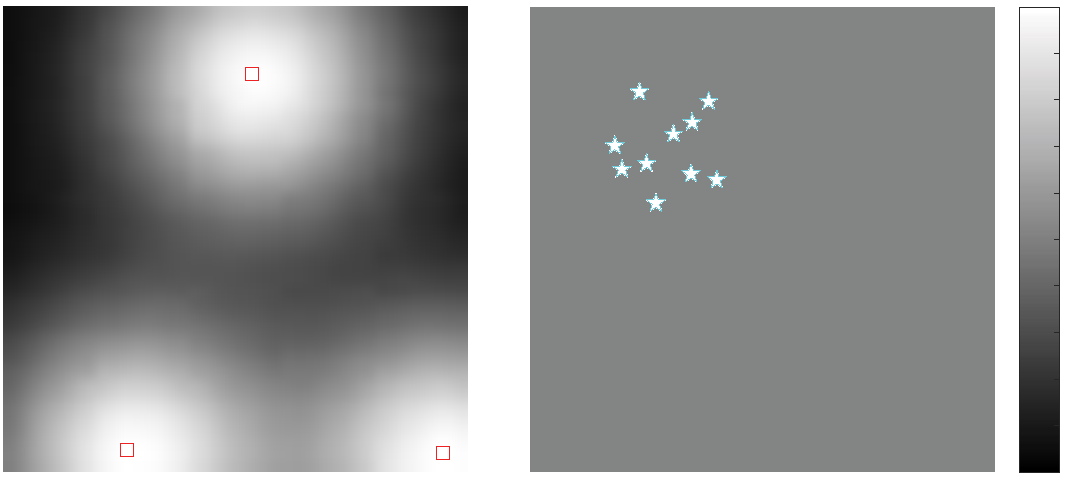
\includegraphics[width=3.4in]{figure/init_10_deploy_pdf}
	\caption{Left: the expected target intensity (the ground truth), right: initial configuration of 10 robots where background color (gray) shows spatial density for every target is uniform. Squares in the left are the peaks of the mixture of Gaussians, and stars on the right are the robots' locations} 
	\label{fig:fig1}
\end{figure}

\begin{figure}
	\centering
	 \begin{subfigure}[b]{0.22\textwidth}
	\centering
	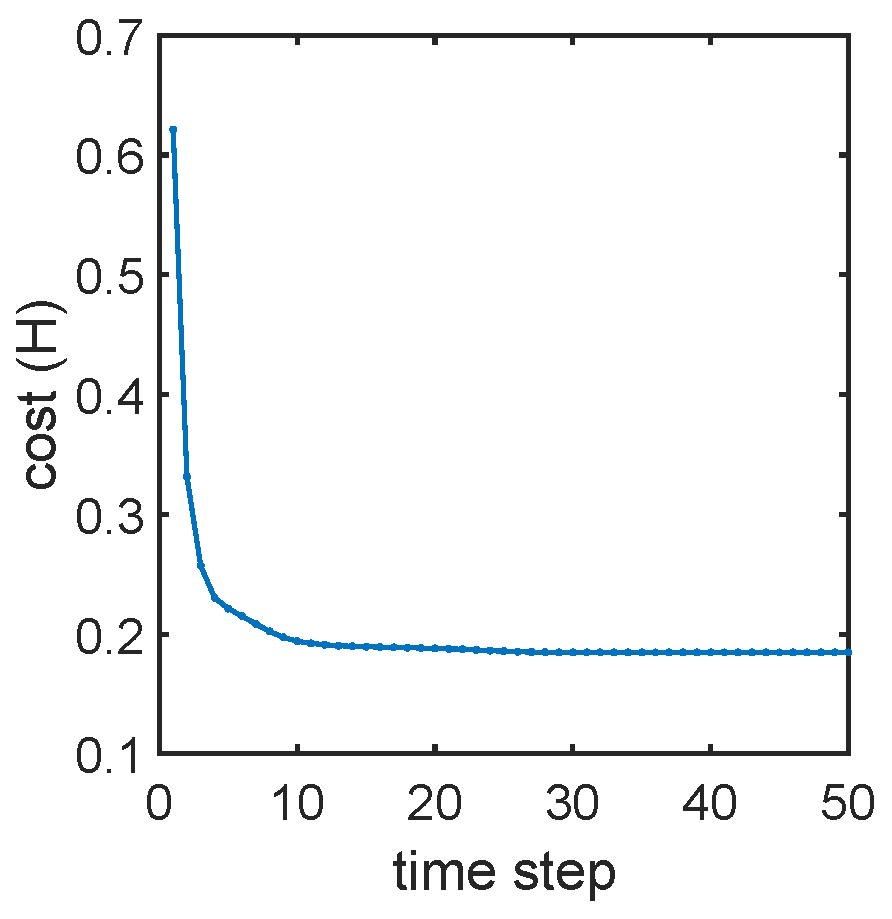
\includegraphics[width=1.5in]{figure/init_10_deploy_cmd2}
	\caption{}
	\end{subfigure}	
	 \begin{subfigure}[b]{0.22\textwidth}
	\centering
	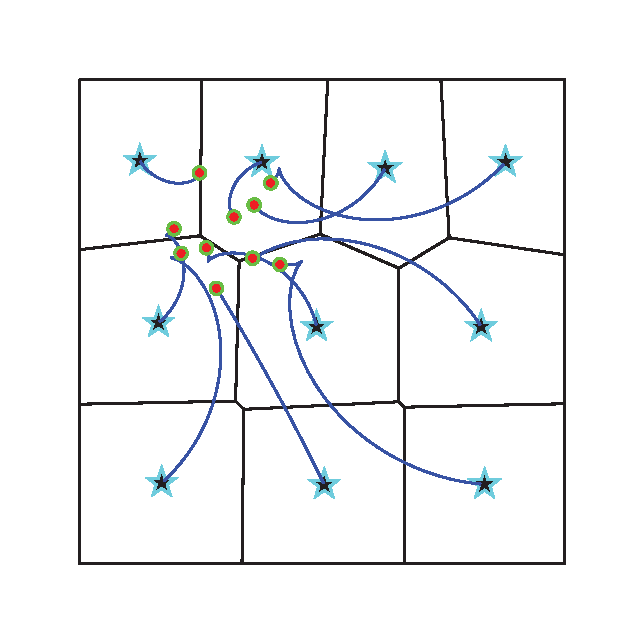
\includegraphics[width=1.69in]{figure/init_10_deploy_cmd1}
	%	\caption{$k=1$}
	\caption{}
\end{subfigure}	
%	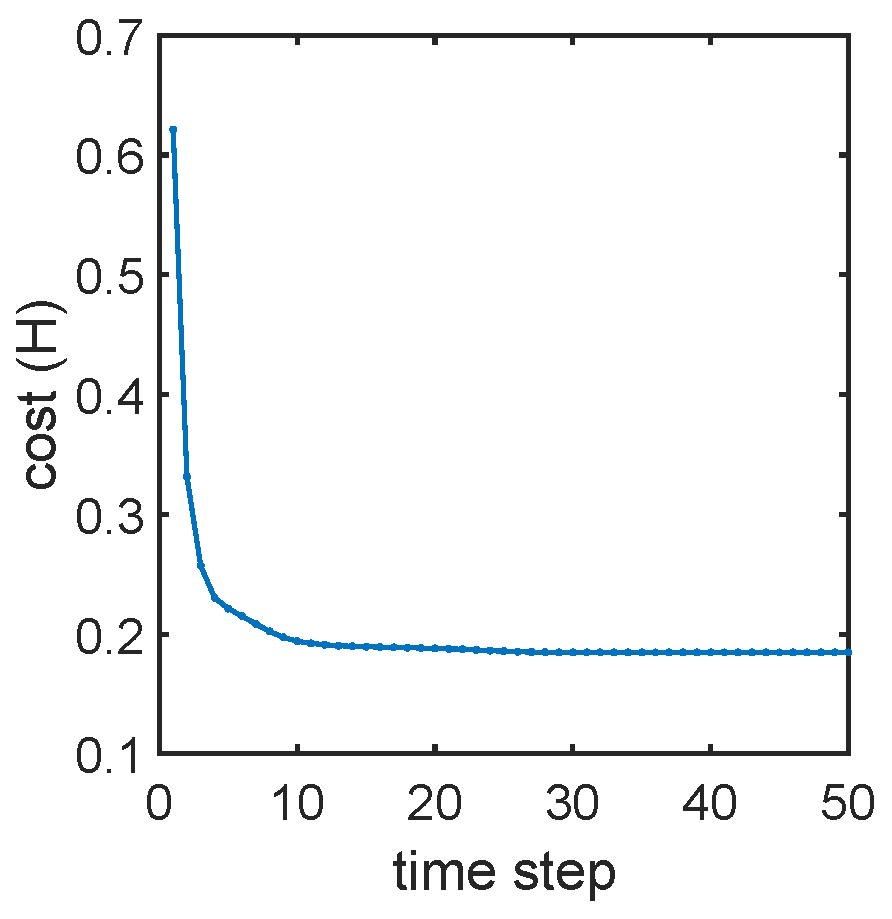
\includegraphics[width=3.4in]{figure/init_10_deploy_cmd2}
	\caption{One-time deployment, (a) cost change during Algorithm 1, (b) optimal path respecting unicycle kinematic constraint (small circles: initial positions, stars: target positions, solid lines: partitions at target positions)}
	\label{fig:fig2}
\end{figure}
\begin{figure}
	\centering
	 \begin{subfigure}[b]{0.169\textwidth}
	 	\centering
		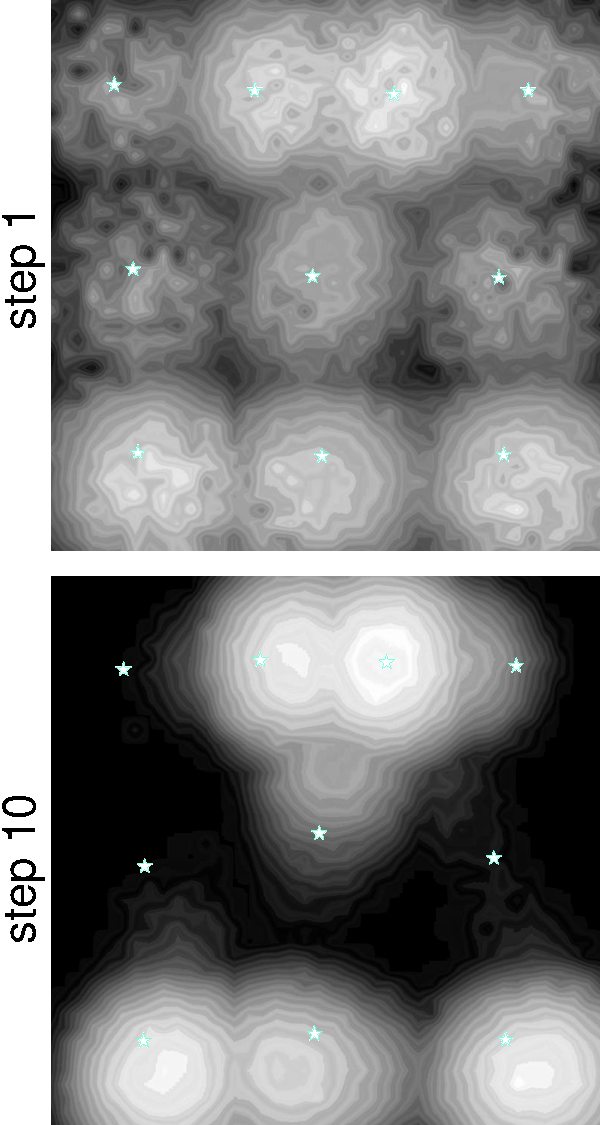
\includegraphics[width=1.093in]{figure/order1_step_0110_pdf}
		\caption{$k=1$}
	\end{subfigure}
	\begin{subfigure}[b]{0.15\textwidth}
		\centering
		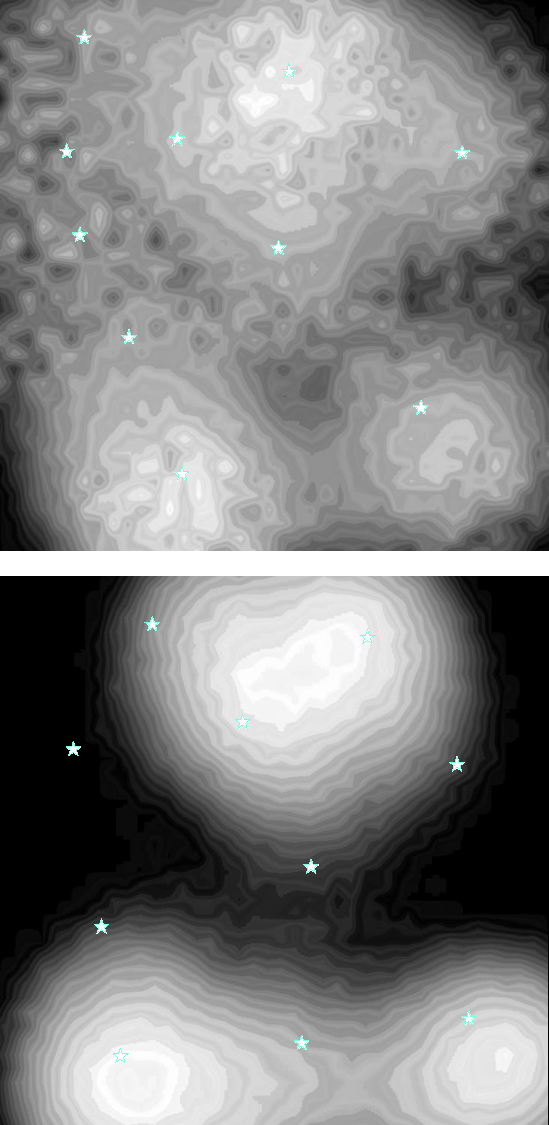
\includegraphics[width=1in]{figure/order2_step_0110_pdf}
		\caption{$k=2$}
	\end{subfigure}
	 \begin{subfigure}[b]{0.15\textwidth}
	\centering
	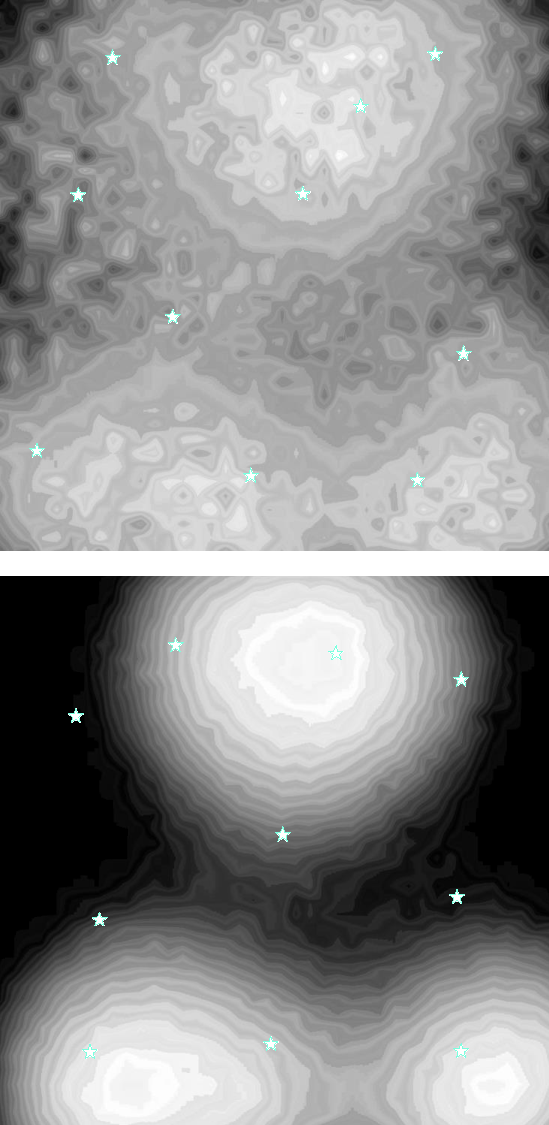
\includegraphics[width=1in]{figure/ordern_step_0110_pdf}
	\caption{$k=10$}
\end{subfigure}
	\caption{Belief propagation using various methods with moderate detection range where $\Sigma_B = 0.04\mathbf{I}$ ((a) $k=1$, (b) $k=2$, (c) $k=10$, the 1st row: step 1, the 2nd row: step 10, stars: positions of robots at $10^{\text{th}}$ step)}
	\label{fig:fig3}
\end{figure}

\textit{Convergence of deployment algorithm:}
First, the behavior of the deployment strategy is discussed. Given the initial uniform prior belief, robots is governed by the gradient descent strategy (Algorithm \ref{alg1}) to obtain the next way-point $x_1$ for the next time step $1$. As previously noted in the Section \ref{sec:sec5}, robots move toward the locations which maximize the likelihood of positive detections.
Fig. \ref{fig:fig2}(a) shows the convergence of the algorithm, and Fig. \ref{fig:fig2}(b) illustrates the path generated by optimal control low when each robot has unicycle kinematics. 

\textit{Filtering performance:}
Next, we present the evolution of the object map given the uniform, initial map (Fig. \ref{fig:fig1}(right)) with successive positive observations, each followed by the gradient descent strategy and filtering process. Fig. \ref{fig:fig3} illustrates the map building process, by different methods with $k=1,\,2,\,10$ respectively, given a moderate covariance values $\Sigma_B = 0.04\mathbf{I}$ for the binary detection where $\mathbf{I} \in \mathbb{R}^{d\times d}$ is an identity matrix, by showing robots' positions and the current belief at time step $1$ and $10$ respectively.
The results in figures clearly show that the coordinated strategies ($k=2,\,10$) yields relatively better mapping results than non-coordinated strategy $k=1$ compared to the ground truth map shown in Fig \ref{fig:fig1}(left).
In addition, Fig. \ref{fig:fig5} compares the K-L divergence values 
between different strategies during the evolution. Fig. \ref{fig:fig5} also includes the case when robots are stationary\footnote{The robots do not change their positions over time, and simply collect observations from the initial locations (as depicted in Fig. \ref{fig:fig1}(right)).} merely to illustrate the pure filtering performance.  As can be seen, our deployment strategy has noticeably improved the quality of the map retrieval for all cases.
The occurrence of sudden jumps (between the time step 0 and 1) in the K-L divergence values observed in Fig \ref{fig:fig5}(a) demonstrates the cases when the initial uniform density happened to a better `\emph{guess}' than the crude belief obtained after a single propagation of the filtering process.
\begin{figure}
	\centering
	\begin{subfigure}[b]{0.23\textwidth}
		\centering
		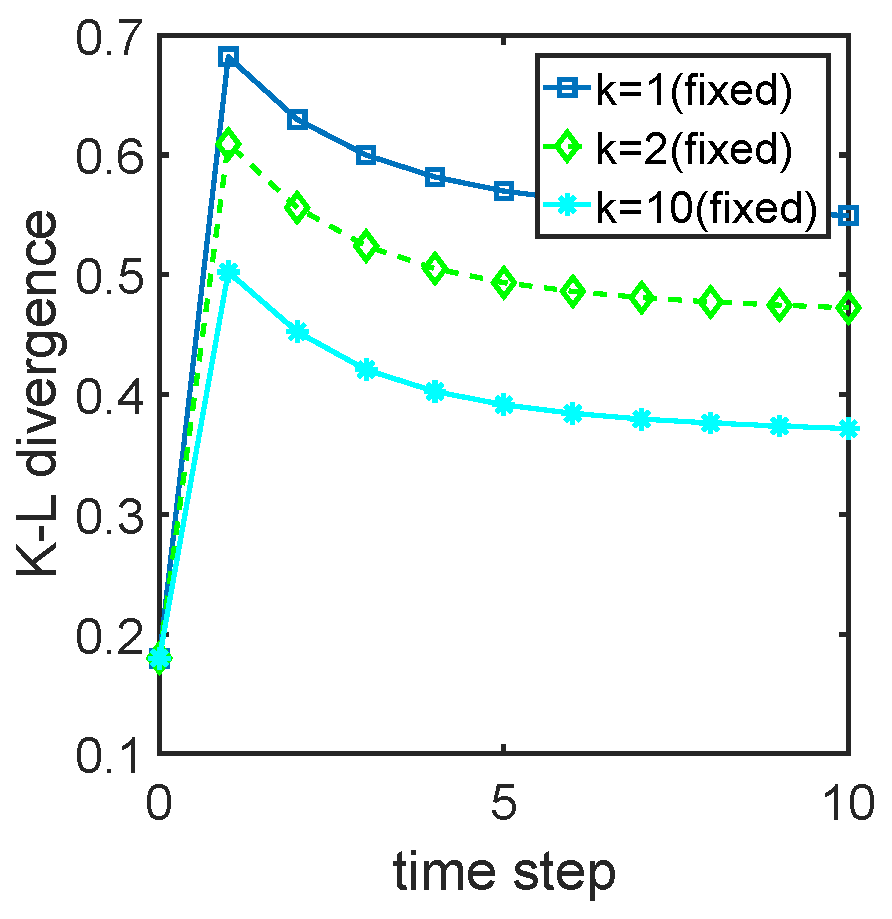
\includegraphics[width=1.7in]{figure/kl_div_2}
		\caption{}
	\end{subfigure}
	\begin{subfigure}[b]{0.23\textwidth}
		\centering
		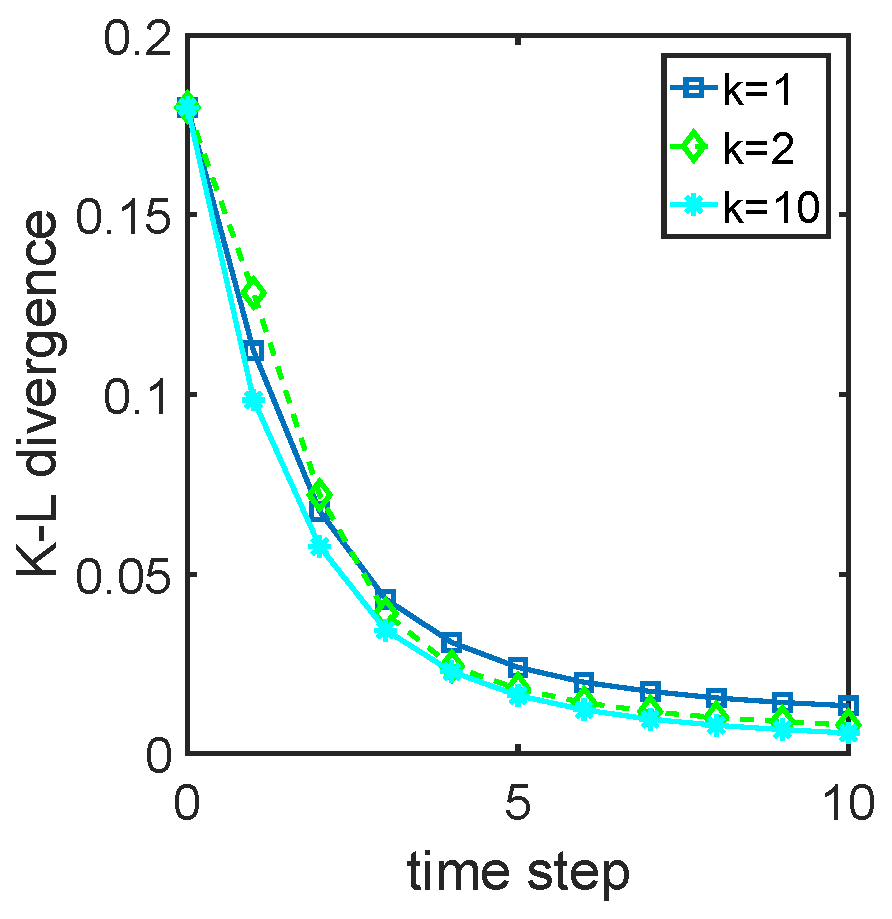
\includegraphics[width=1.7in]{figure/kl_div_1}
		\caption{}
	\end{subfigure}
	\caption{Comparison of K-L divergence from the actual distribution between different sensor models during belief propagation; (a) robots are stationary, (b) robots are deployed via gradient algorithm}
	\label{fig:fig5}
\end{figure}
\begin{figure}
	\centering
	\begin{subfigure}[b]{0.15\textwidth}
		\centering
		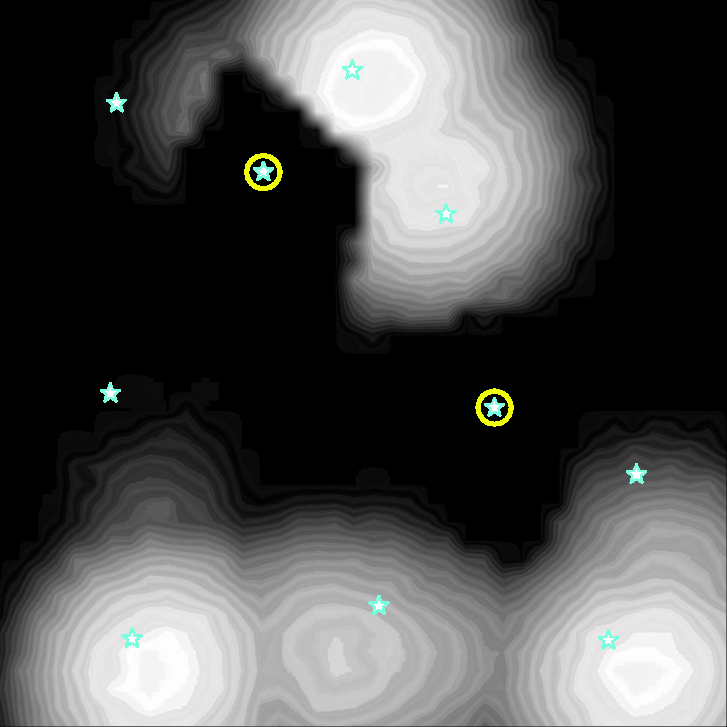
\includegraphics[width=1in]{figure/fault_order_1_pdf}
		\caption{$k=1$}
	\end{subfigure}
	\begin{subfigure}[b]{0.15\textwidth}
		\centering
		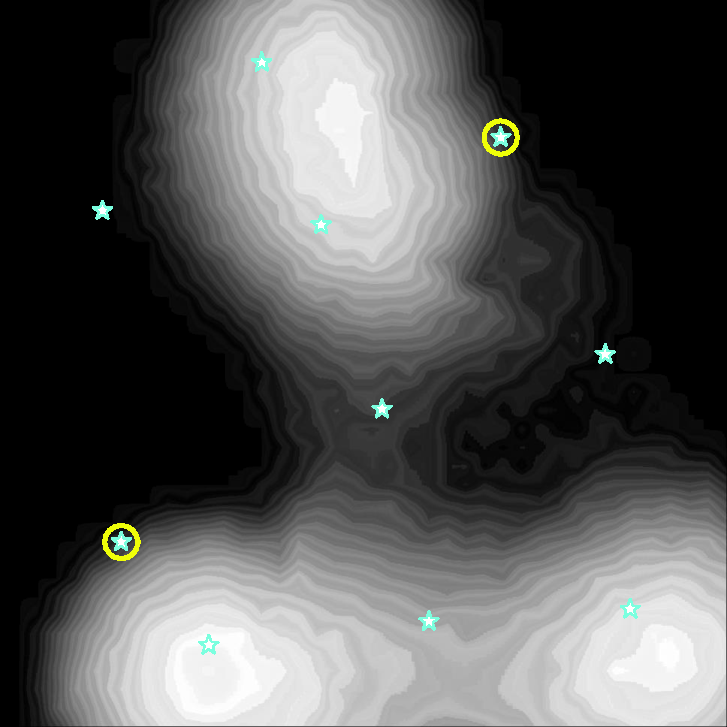
\includegraphics[width=1in]{figure/fault_order_2_pdf}
		\caption{$k=2$}
	\end{subfigure}
	\begin{subfigure}[b]{0.15\textwidth}
	\centering
	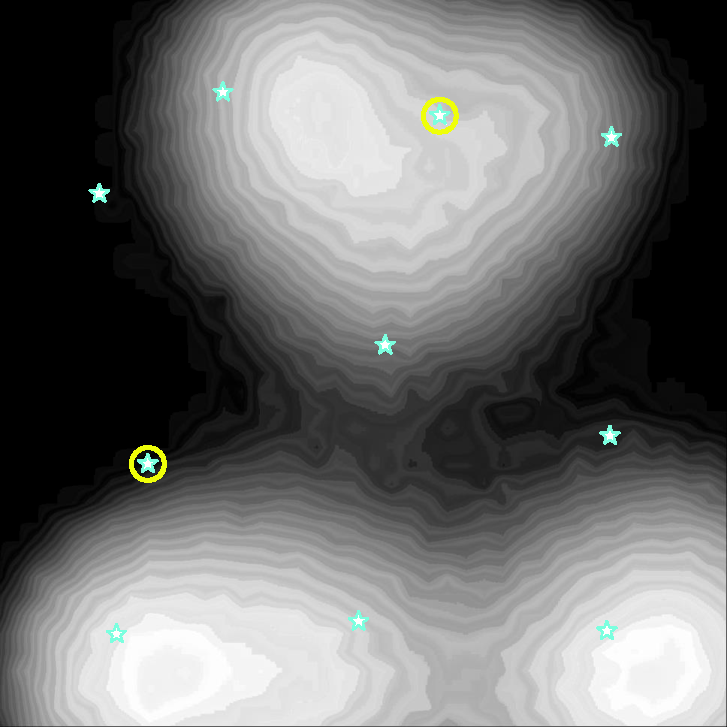
\includegraphics[width=1in]{figure/fault_order_n_pdf}
	\caption{$k=10$}
\end{subfigure}
	\caption{Comparison of robots' configuration and beliefs at the final step with two approaches, $k=1, \,2,\,10$ when two of the sensors fails (circled) and $\Sigma_B = 0.04\mathbf{I}$ for both cases }
	\label{fig:fig6}
\end{figure}
\begin{figure}
	\centering
	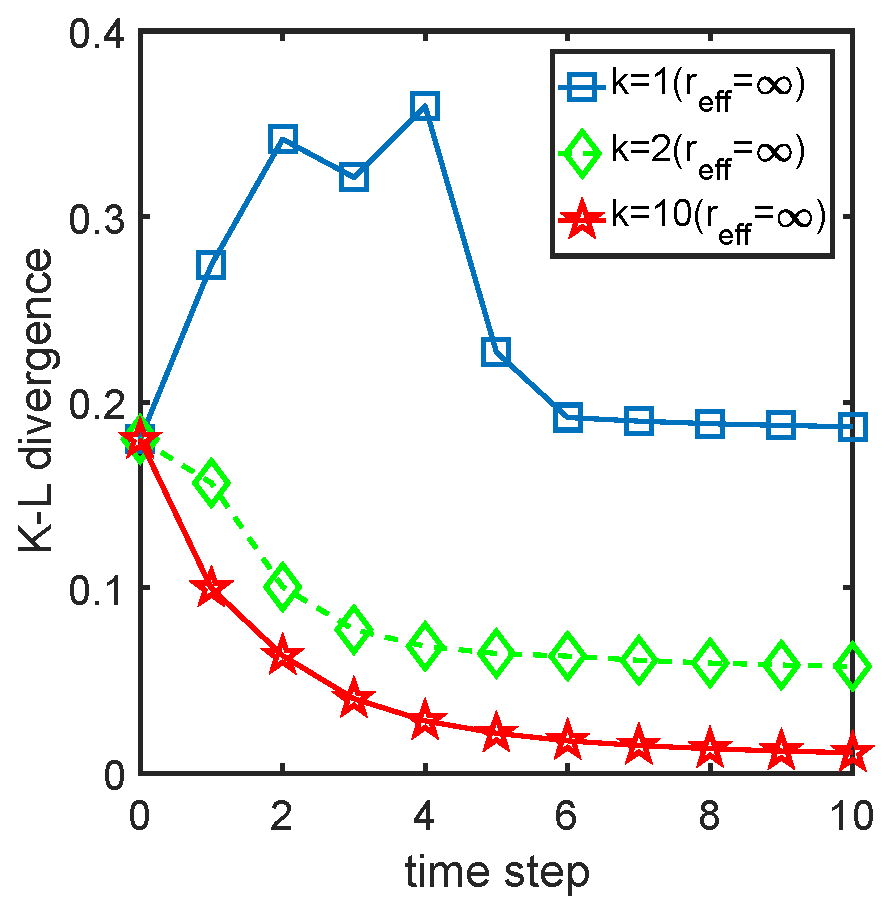
\includegraphics[width=1.67in]{figure/fault_kl2}
	\caption{Comparison of K-L divergence from the ground-truth distribution between multiple strategies ($k=1,\,2,\,10$), when two sensors fail, during the evolution}
	\label{fig:fig7}
\end{figure}

\textit{Robustness to sensor failure:}
As seen in the previous section, the performance gain by the coordinated methods over the non-coordinated method ($k=1$) is not large enough to trade-off the increased sensing cost.
This section presents an example when the coordinated strategy becomes more desirable. And, this happens when the sensors are not perfect and likely to fail to detect a target. 
Results for configurations and spatial distributions after $10^{\textup{th}}$ step with $k=1,\,2,\,10$, are shown in Fig. \ref{fig:fig6}(a)-(c), respectively.  
As can be seen from Fig \ref{fig:fig6} and Fig. \ref{fig:fig7}, the map retrieved by the coordinated strategies $k=2,\,10$ are more accurate, and more robust to the sensor failure compared to that obtained with the non-coordinated strategy. 
Due to its fully decentralized nature of the sensor model, it is not surprising to see from this example that the non-coordinated method works poorly under the sensor failures. 

\section{An example: Precipitation Mapping using Windshield Wiper Data}
\label{sec:sec8}
Existing methods for precipitation measurements (e.g., weather radar, stationary rain guages, etc) usually do not pose high enough temporal resolution for building a precipitation map to be used for time critical hydrological applications, such as, urban flash floods monitoring. In this section, we provide an example based on real-world data which shows that our Bayesian update scheme can be used for online precipitation mapping via utilizing the multi-vehicles' real-time windshield wiper data, which is spatially precise, and has much higher temporal resolution than the data collected from other sources.
The vehicle wiper dataset---obtained from the University
of Michigan Transportation Research Institute
(UMTRI)---contains vehicle locations along with their wiper
intensity data (four normalized intensity modes: $0,0.33,0.66,1$) which is generated at every 2ms. The windshield wiper data is collected from up to 69 vehicles. 
 We consider a rainfall event occurred at the city of Ann Arbor between 21:47 and 22:26 on August 11th in 2014 (in UTC time). As shown in Fig \ref{fig:fig8}, the rectangular area, $[-83.8,-83.66] \times [42.22,42.34]$ (longitude, latitude in GPS coordinates, respectively) contains the boundary of Ann Arbor, which is drawn by lines. We assume that driver in each vehicle turns on the windshield wiper when detecting rain, and turns it off, otherwise, immediately in both cases. In addition, each driver is assumed to be capable of detecting rain from up to $1$ mile away from the source of rain (i.e., $r_{\textup{eff}} = 1$). We consider a product of two Gaussians---one with covariance matrices $\mathbf{I}$ (unit: mile) for detection, and the other with $0.5\mathbf{I}$ (unit: normalized wiper intensity) for the intensity measurement, respectively---as the windshield wiper sensor model. Since, we did not have control over the vehicles at the time, the map is updated merely using the passively gathered windshield wiper measurements without utilizing our deployment algorithm, namely, Algorithm \ref{alg1}. For our algorithm, the initial expected wind wiper intensity is uniformly set to $0.3$ out of $1$ over the whole region. 
Fig \ref{fig:fig8} shows two time series of precipitation maps generated by the two different methods where we the wiper data is sampled at every 1 second, and the radar is sampled at every 5 minute.
The 1st row of Fig. \ref{fig:fig8} shows incremental mapping by our method (non-coordinated strategy, $k=1$). The color intensity shows the relative windshield wiper intensity where brighter area implies relatively more precipitation, and the black area means no precipitation\footnote{We have experimentally validated that there are very strong correlation between windshield wiper intensity and the actual precipitation rate by comparing the windshield wiper data and visual data from the in-vehicle mounted camera.}
The figures shown in the 2nd row of Fig. \ref{fig:fig8} illustrates the instantaneous precipitation rate measured by the 
NOAA Next Generation Radar Level III (NEXRAD-III).
The radar is a Doppler type which is located at Detroit, the nearest NOAA's station to the city of Ann Arbor. 
%The windshield wiper measurements do not provide the specific  precipitation data as the radar does, nevertheless, the color intensities was used to compare the difference between the two maps.

The rough visual correlation that is shown between the two series of maps shown in Fig \ref{fig:fig8}, especially at the later time (22:26:00) is, unfortunately, not sufficient to validate the real-world performance of our method. 
There can be numerous reasons for the dissimilarity between the two. In the following, we will discuss a few of them briefly. First, weather radar observations are known to frequently provide unreliable information, e.g., due to blocking or deflection of radar beam, non-precipitation echo (see, e.g., \cite{berg2016creation} to find more details on this topic). In other words, the radar measurements are not consistent enough to be used as the ground truth precipitation data.
Second, relative to the size of the region of interest, the number of vehicle (only up to 4 vehicles were active during the rainfall event shown in this example) is not large enough to capture the spatial rainfall distribution reasonably well.
Lastly, our assumption on the effective sensor range for drivers could have been either too restrictive or unrealistic.


\begin{figure}
	\centering
	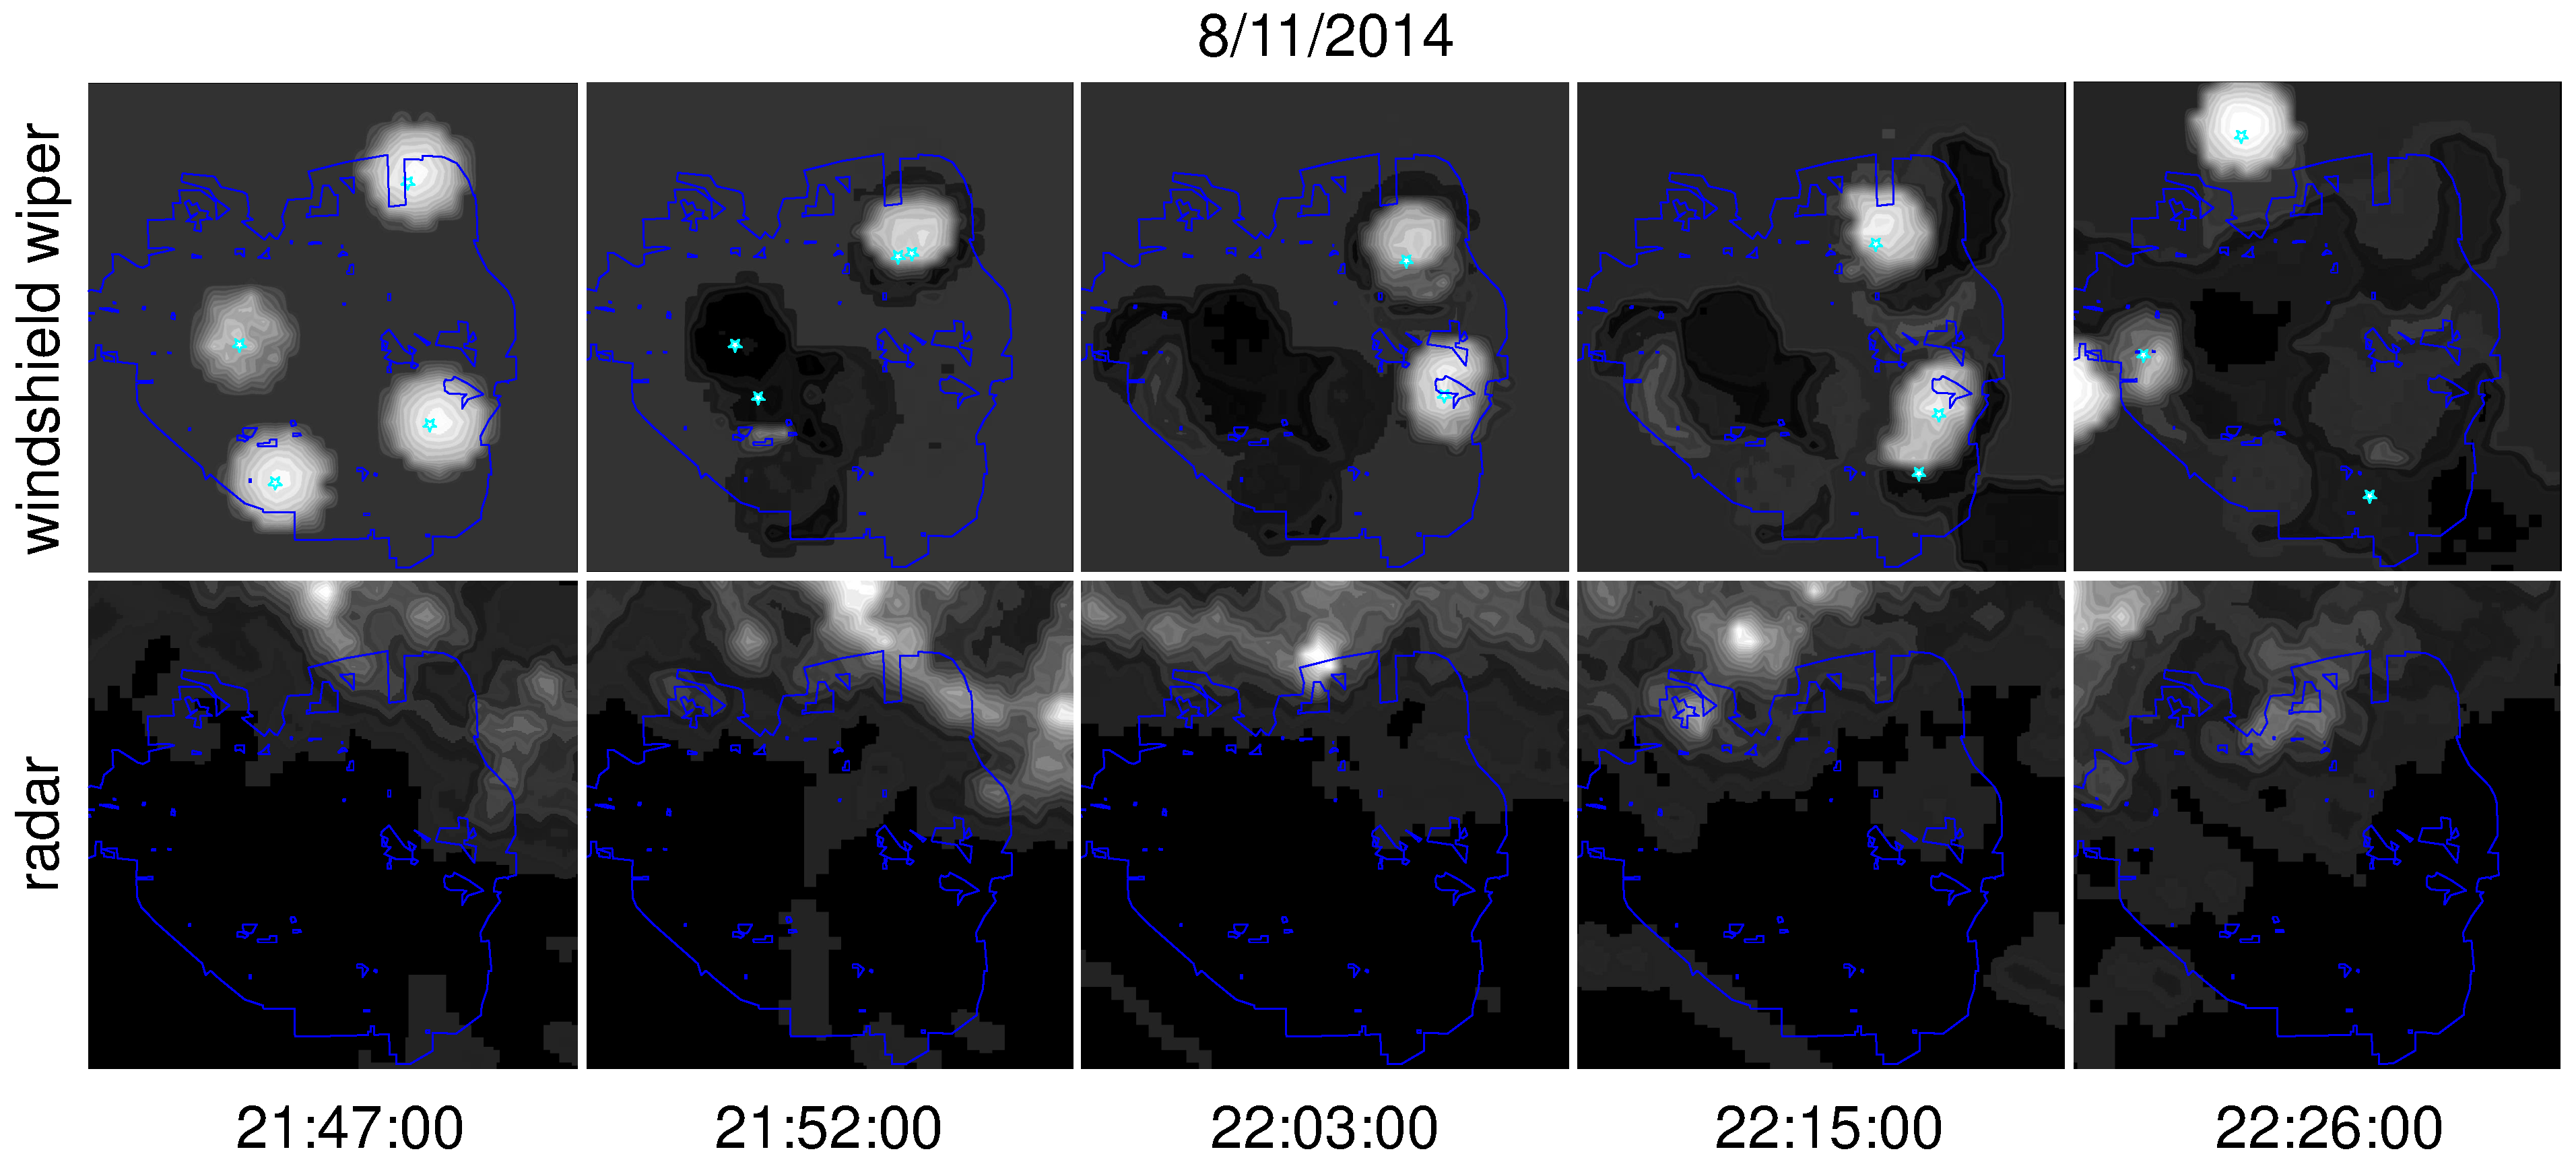
\includegraphics[width=3.5in]{figure/wind_wiper_data3}
	\caption{A time series of precipitation map build by windshield wiper data collected from up to 4 vehicles using our Bayesian estimator (top row) vs a time series of map built by instantaneous precipitation rate measurements from NEXRAD-III (bottom row). Both maps are generated over the city of Ann Arbor, MI, USA (lines: boundary of the city, stars: vehicles' locations, color intensity: relative precipitation rate where the maximum precipitation rate by the radar is 2in/hr)}
	\label{fig:fig8}
\end{figure}


\section{Conclusions and Future Work}
\label{sec:sec9}
In this paper, we have presented a general deployment strategy for a fleet of autonomous vehicles for maximum recovery of spatial distribution map over a bounded space. It is expected that our method will fail if there are not enough number of mobile agents having long enough effective sensing ranges relative to the workspace size. One of our future works is, therefore, to develop multi-agent patrolling algorithms (see e.g., \cite{portugal2011survey}) to compensate such problems where there are not enough number of sensors to cover the whole target space.
Also, as reported in the literature \cite{anguelov2004detecting}, our combined sensor model can be used to model the real-world laser scanner's behavior, nevertheless, it is one of our future works to conduct extensive real world multi-robot experiments for further validation of our range sensor model.
Lastly, we assumed in this study that the beliefs are shared between robots such that both tasks of propagating and approximating belief require a central entity. It is one of our future works to devise distributed communication protocol to enable distributed belief estimation. 
%\section{type of sensors}

\bibliographystyle{IEEEtran}
\bibliography{reference_park_17}

% that's all folks
\end{document}


